\documentclass[class=minimal,border=0pt]{standalone}
\usepackage{hyperref}
\hypersetup{
colorlinks=true,
urlcolor=cyan}
\usepackage{tikz}
\begin{document}
%\documentclass{standalone}
%\usepackage{tikz}
%\usetikzlibrary{patterns,plotmarks}
%\begin{document}
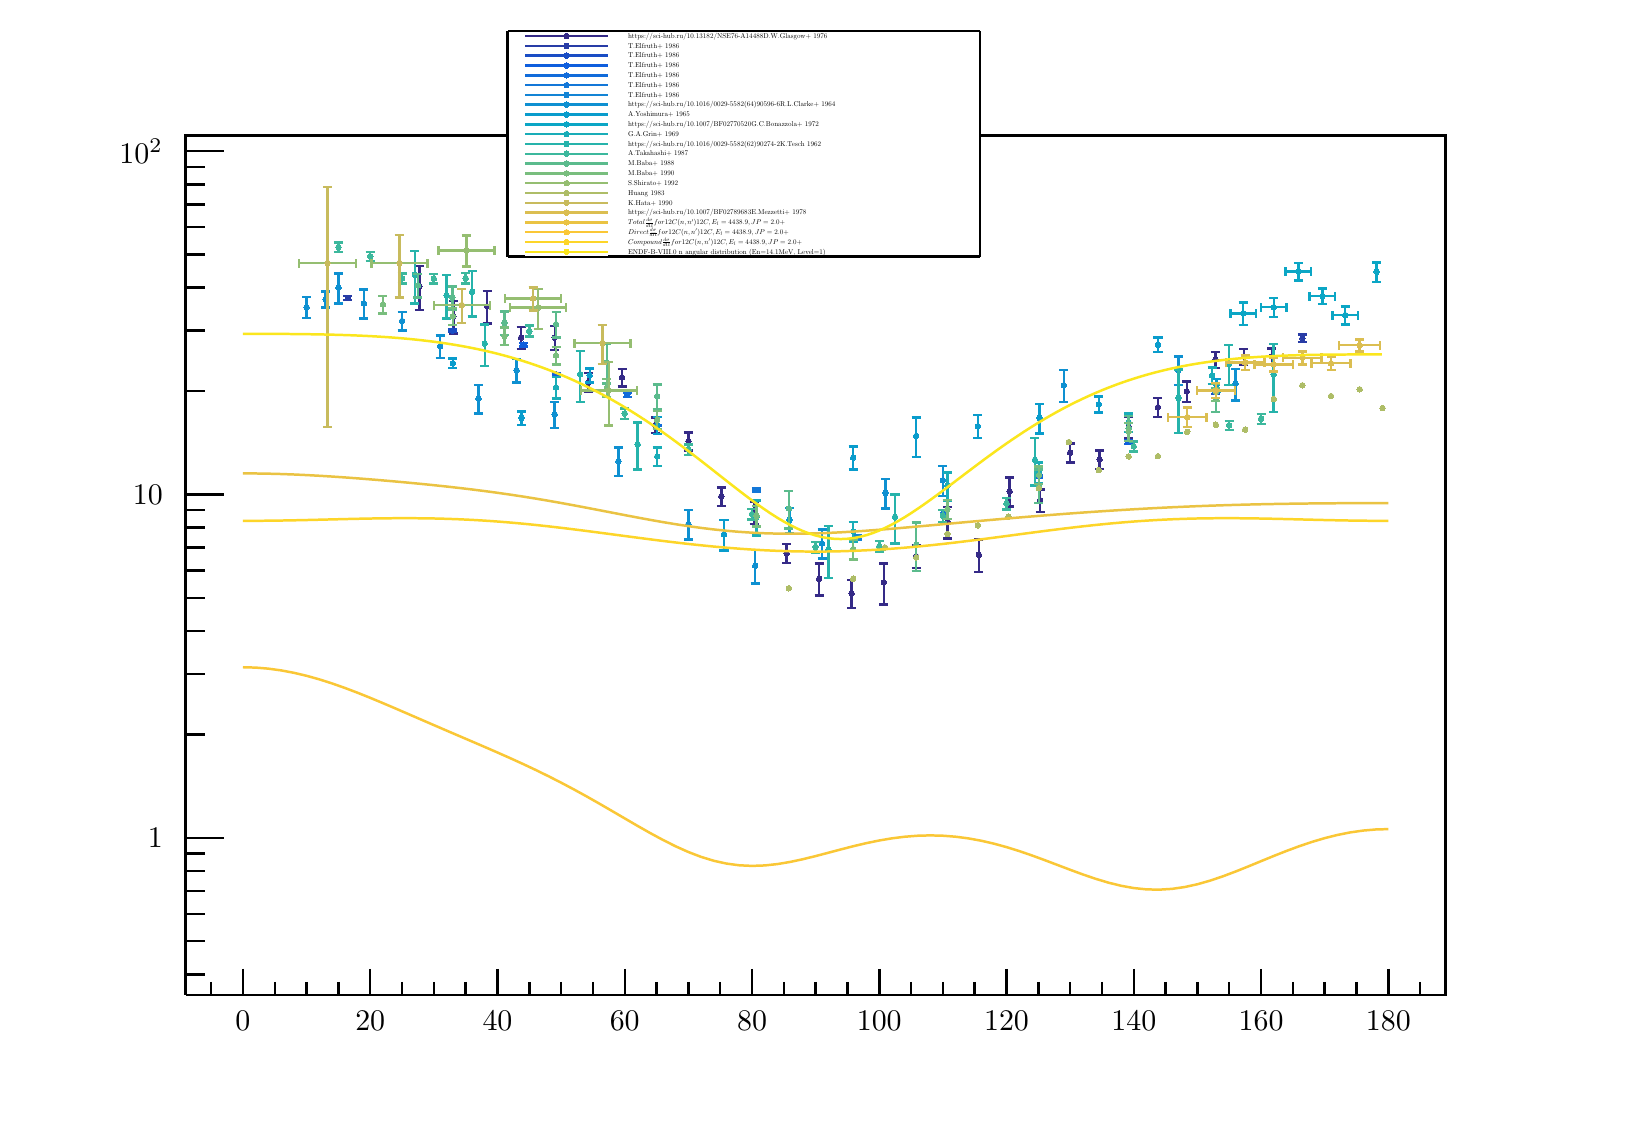
\begin{tikzpicture}
\def\CheckTikzLibraryLoaded#1{ \ifcsname tikz@library@#1@loaded\endcsname \else \PackageWarning{tikz}{usetikzlibrary{#1} is missing in the preamble.} \fi }
\CheckTikzLibraryLoaded{patterns}
\CheckTikzLibraryLoaded{plotmarks}
\pgfdeclareplotmark{cross} {
\pgfpathmoveto{\pgfpoint{-0.3\pgfplotmarksize}{\pgfplotmarksize}}
\pgfpathlineto{\pgfpoint{+0.3\pgfplotmarksize}{\pgfplotmarksize}}
\pgfpathlineto{\pgfpoint{+0.3\pgfplotmarksize}{0.3\pgfplotmarksize}}
\pgfpathlineto{\pgfpoint{+1\pgfplotmarksize}{0.3\pgfplotmarksize}}
\pgfpathlineto{\pgfpoint{+1\pgfplotmarksize}{-0.3\pgfplotmarksize}}
\pgfpathlineto{\pgfpoint{+0.3\pgfplotmarksize}{-0.3\pgfplotmarksize}}
\pgfpathlineto{\pgfpoint{+0.3\pgfplotmarksize}{-1.\pgfplotmarksize}}
\pgfpathlineto{\pgfpoint{-0.3\pgfplotmarksize}{-1.\pgfplotmarksize}}
\pgfpathlineto{\pgfpoint{-0.3\pgfplotmarksize}{-0.3\pgfplotmarksize}}
\pgfpathlineto{\pgfpoint{-1.\pgfplotmarksize}{-0.3\pgfplotmarksize}}
\pgfpathlineto{\pgfpoint{-1.\pgfplotmarksize}{0.3\pgfplotmarksize}}
\pgfpathlineto{\pgfpoint{-0.3\pgfplotmarksize}{0.3\pgfplotmarksize}}
\pgfpathclose
\pgfusepathqstroke
}
\pgfdeclareplotmark{cross*} {
\pgfpathmoveto{\pgfpoint{-0.3\pgfplotmarksize}{\pgfplotmarksize}}
\pgfpathlineto{\pgfpoint{+0.3\pgfplotmarksize}{\pgfplotmarksize}}
\pgfpathlineto{\pgfpoint{+0.3\pgfplotmarksize}{0.3\pgfplotmarksize}}
\pgfpathlineto{\pgfpoint{+1\pgfplotmarksize}{0.3\pgfplotmarksize}}
\pgfpathlineto{\pgfpoint{+1\pgfplotmarksize}{-0.3\pgfplotmarksize}}
\pgfpathlineto{\pgfpoint{+0.3\pgfplotmarksize}{-0.3\pgfplotmarksize}}
\pgfpathlineto{\pgfpoint{+0.3\pgfplotmarksize}{-1.\pgfplotmarksize}}
\pgfpathlineto{\pgfpoint{-0.3\pgfplotmarksize}{-1.\pgfplotmarksize}}
\pgfpathlineto{\pgfpoint{-0.3\pgfplotmarksize}{-0.3\pgfplotmarksize}}
\pgfpathlineto{\pgfpoint{-1.\pgfplotmarksize}{-0.3\pgfplotmarksize}}
\pgfpathlineto{\pgfpoint{-1.\pgfplotmarksize}{0.3\pgfplotmarksize}}
\pgfpathlineto{\pgfpoint{-0.3\pgfplotmarksize}{0.3\pgfplotmarksize}}
\pgfpathclose
\pgfusepathqfillstroke
}
\pgfdeclareplotmark{newstar} {
\pgfpathmoveto{\pgfqpoint{0pt}{\pgfplotmarksize}}
\pgfpathlineto{\pgfqpointpolar{44}{0.5\pgfplotmarksize}}
\pgfpathlineto{\pgfqpointpolar{18}{\pgfplotmarksize}}
\pgfpathlineto{\pgfqpointpolar{-20}{0.5\pgfplotmarksize}}
\pgfpathlineto{\pgfqpointpolar{-54}{\pgfplotmarksize}}
\pgfpathlineto{\pgfqpointpolar{-90}{0.5\pgfplotmarksize}}
\pgfpathlineto{\pgfqpointpolar{234}{\pgfplotmarksize}}
\pgfpathlineto{\pgfqpointpolar{198}{0.5\pgfplotmarksize}}
\pgfpathlineto{\pgfqpointpolar{162}{\pgfplotmarksize}}
\pgfpathlineto{\pgfqpointpolar{134}{0.5\pgfplotmarksize}}
\pgfpathclose
\pgfusepathqstroke
}
\pgfdeclareplotmark{newstar*} {
\pgfpathmoveto{\pgfqpoint{0pt}{\pgfplotmarksize}}
\pgfpathlineto{\pgfqpointpolar{44}{0.5\pgfplotmarksize}}
\pgfpathlineto{\pgfqpointpolar{18}{\pgfplotmarksize}}
\pgfpathlineto{\pgfqpointpolar{-20}{0.5\pgfplotmarksize}}
\pgfpathlineto{\pgfqpointpolar{-54}{\pgfplotmarksize}}
\pgfpathlineto{\pgfqpointpolar{-90}{0.5\pgfplotmarksize}}
\pgfpathlineto{\pgfqpointpolar{234}{\pgfplotmarksize}}
\pgfpathlineto{\pgfqpointpolar{198}{0.5\pgfplotmarksize}}
\pgfpathlineto{\pgfqpointpolar{162}{\pgfplotmarksize}}
\pgfpathlineto{\pgfqpointpolar{134}{0.5\pgfplotmarksize}}
\pgfpathclose
\pgfusepathqfillstroke
}
\definecolor{c}{rgb}{1,1,1};
\draw [color=c, fill=c] (0,0) rectangle (20,13.639);
\draw [color=c, fill=c] (2,1.3639) rectangle (18,12.2751);
\definecolor{c}{rgb}{0,0,0};
\draw [c,line width=0.9] (2,1.3639) -- (2,12.2751) -- (18,12.2751) -- (18,1.3639) -- (2,1.3639);
\draw [c,line width=0.9] (2,1.3639) -- (18,1.3639);
\draw [c,line width=0.9] (2.72727,1.69123) -- (2.72727,1.3639);
\draw [c,line width=0.9] (3.13131,1.52756) -- (3.13131,1.3639);
\draw [c,line width=0.9] (3.53535,1.52756) -- (3.53535,1.3639);
\draw [c,line width=0.9] (3.93939,1.52756) -- (3.93939,1.3639);
\draw [c,line width=0.9] (4.34343,1.69123) -- (4.34343,1.3639);
\draw [c,line width=0.9] (4.74747,1.52756) -- (4.74747,1.3639);
\draw [c,line width=0.9] (5.15152,1.52756) -- (5.15152,1.3639);
\draw [c,line width=0.9] (5.55556,1.52756) -- (5.55556,1.3639);
\draw [c,line width=0.9] (5.9596,1.69123) -- (5.9596,1.3639);
\draw [c,line width=0.9] (6.36364,1.52756) -- (6.36364,1.3639);
\draw [c,line width=0.9] (6.76768,1.52756) -- (6.76768,1.3639);
\draw [c,line width=0.9] (7.17172,1.52756) -- (7.17172,1.3639);
\draw [c,line width=0.9] (7.57576,1.69123) -- (7.57576,1.3639);
\draw [c,line width=0.9] (7.9798,1.52756) -- (7.9798,1.3639);
\draw [c,line width=0.9] (8.38384,1.52756) -- (8.38384,1.3639);
\draw [c,line width=0.9] (8.78788,1.52756) -- (8.78788,1.3639);
\draw [c,line width=0.9] (9.19192,1.69123) -- (9.19192,1.3639);
\draw [c,line width=0.9] (9.59596,1.52756) -- (9.59596,1.3639);
\draw [c,line width=0.9] (10,1.52756) -- (10,1.3639);
\draw [c,line width=0.9] (10.404,1.52756) -- (10.404,1.3639);
\draw [c,line width=0.9] (10.8081,1.69123) -- (10.8081,1.3639);
\draw [c,line width=0.9] (11.2121,1.52756) -- (11.2121,1.3639);
\draw [c,line width=0.9] (11.6162,1.52756) -- (11.6162,1.3639);
\draw [c,line width=0.9] (12.0202,1.52756) -- (12.0202,1.3639);
\draw [c,line width=0.9] (12.4242,1.69123) -- (12.4242,1.3639);
\draw [c,line width=0.9] (12.8283,1.52756) -- (12.8283,1.3639);
\draw [c,line width=0.9] (13.2323,1.52756) -- (13.2323,1.3639);
\draw [c,line width=0.9] (13.6364,1.52756) -- (13.6364,1.3639);
\draw [c,line width=0.9] (14.0404,1.69123) -- (14.0404,1.3639);
\draw [c,line width=0.9] (14.4444,1.52756) -- (14.4444,1.3639);
\draw [c,line width=0.9] (14.8485,1.52756) -- (14.8485,1.3639);
\draw [c,line width=0.9] (15.2525,1.52756) -- (15.2525,1.3639);
\draw [c,line width=0.9] (15.6566,1.69123) -- (15.6566,1.3639);
\draw [c,line width=0.9] (16.0606,1.52756) -- (16.0606,1.3639);
\draw [c,line width=0.9] (16.4646,1.52756) -- (16.4646,1.3639);
\draw [c,line width=0.9] (16.8687,1.52756) -- (16.8687,1.3639);
\draw [c,line width=0.9] (17.2727,1.69123) -- (17.2727,1.3639);
\draw [c,line width=0.9] (2.72727,1.69123) -- (2.72727,1.3639);
\draw [c,line width=0.9] (2.32323,1.52756) -- (2.32323,1.3639);
\draw [c,line width=0.9] (17.2727,1.69123) -- (17.2727,1.3639);
\draw [c,line width=0.9] (17.6768,1.52756) -- (17.6768,1.3639);
\draw [anchor=base] (2.72727,0.913811) node[scale=1.08185, color=c, rotate=0]{0};
\draw [anchor=base] (4.34343,0.913811) node[scale=1.08185, color=c, rotate=0]{20};
\draw [anchor=base] (5.9596,0.913811) node[scale=1.08185, color=c, rotate=0]{40};
\draw [anchor=base] (7.57576,0.913811) node[scale=1.08185, color=c, rotate=0]{60};
\draw [anchor=base] (9.19192,0.913811) node[scale=1.08185, color=c, rotate=0]{80};
\draw [anchor=base] (10.8081,0.913811) node[scale=1.08185, color=c, rotate=0]{100};
\draw [anchor=base] (12.4242,0.913811) node[scale=1.08185, color=c, rotate=0]{120};
\draw [anchor=base] (14.0404,0.913811) node[scale=1.08185, color=c, rotate=0]{140};
\draw [anchor=base] (15.6566,0.913811) node[scale=1.08185, color=c, rotate=0]{160};
\draw [anchor=base] (17.2727,0.913811) node[scale=1.08185, color=c, rotate=0]{180};
\draw [c,line width=0.9] (2,1.3639) -- (2,12.2751);
\draw [c,line width=0.9] (2.24,1.62259) -- (2,1.62259);
\draw [c,line width=0.9] (2.24,2.04516) -- (2,2.04516);
\draw [c,line width=0.9] (2.24,2.39043) -- (2,2.39043);
\draw [c,line width=0.9] (2.24,2.68235) -- (2,2.68235);
\draw [c,line width=0.9] (2.24,2.93523) -- (2,2.93523);
\draw [c,line width=0.9] (2.24,3.15827) -- (2,3.15827);
\draw [c,line width=0.9] (2.48,3.3578) -- (2,3.3578);
\draw [anchor= east] (1.844,3.3578) node[scale=1.08185, color=c, rotate=0]{1};
\draw [c,line width=0.9] (2.24,4.67044) -- (2,4.67044);
\draw [c,line width=0.9] (2.24,5.43828) -- (2,5.43828);
\draw [c,line width=0.9] (2.24,5.98308) -- (2,5.98308);
\draw [c,line width=0.9] (2.24,6.40565) -- (2,6.40565);
\draw [c,line width=0.9] (2.24,6.75092) -- (2,6.75092);
\draw [c,line width=0.9] (2.24,7.04284) -- (2,7.04284);
\draw [c,line width=0.9] (2.24,7.29571) -- (2,7.29571);
\draw [c,line width=0.9] (2.24,7.51876) -- (2,7.51876);
\draw [c,line width=0.9] (2.48,7.71829) -- (2,7.71829);
\draw [anchor= east] (1.844,7.71829) node[scale=1.08185, color=c, rotate=0]{10};
\draw [c,line width=0.9] (2.24,9.03093) -- (2,9.03093);
\draw [c,line width=0.9] (2.24,9.79877) -- (2,9.79877);
\draw [c,line width=0.9] (2.24,10.3436) -- (2,10.3436);
\draw [c,line width=0.9] (2.24,10.7661) -- (2,10.7661);
\draw [c,line width=0.9] (2.24,11.1114) -- (2,11.1114);
\draw [c,line width=0.9] (2.24,11.4033) -- (2,11.4033);
\draw [c,line width=0.9] (2.24,11.6562) -- (2,11.6562);
\draw [c,line width=0.9] (2.24,11.8793) -- (2,11.8793);
\draw [c,line width=0.9] (2.48,12.0788) -- (2,12.0788);
\draw [anchor= east] (1.844,12.0788) node[scale=1.08185, color=c, rotate=0]{$10^{2}$};
\definecolor{c}{rgb}{0.2082,0.1664,0.5293};
\draw [c,line width=0.9] (4.96727,10.3577) -- (4.96727,10.6169);
\draw [c,line width=0.9] (4.90996,10.6169) -- (5.02458,10.6169);
\draw [c,line width=0.9] (4.96727,10.3577) -- (4.96727,10.0574);
\draw [c,line width=0.9] (4.90996,10.0574) -- (5.02458,10.0574);
\draw [c,line width=0.9] (5.39879,9.97811) -- (5.39879,10.1738);
\draw [c,line width=0.9] (5.34148,10.1738) -- (5.45609,10.1738);
\draw [c,line width=0.9] (5.39879,9.97811) -- (5.39879,9.75987);
\draw [c,line width=0.9] (5.34148,9.75987) -- (5.45609,9.75987);
\draw [c,line width=0.9] (5.82868,10.1074) -- (5.82868,10.3034);
\draw [c,line width=0.9] (5.77137,10.3034) -- (5.88599,10.3034);
\draw [c,line width=0.9] (5.82868,10.1074) -- (5.82868,9.88876);
\draw [c,line width=0.9] (5.77137,9.88876) -- (5.88599,9.88876);
\draw [c,line width=0.9] (6.25939,9.70959) -- (6.25939,9.84615);
\draw [c,line width=0.9] (6.20208,9.84615) -- (6.3167,9.84615);
\draw [c,line width=0.9] (6.25939,9.70959) -- (6.25939,9.56242);
\draw [c,line width=0.9] (6.20208,9.56242) -- (6.3167,9.56242);
\draw [c,line width=0.9] (6.68687,9.70959) -- (6.68687,9.85536);
\draw [c,line width=0.9] (6.62956,9.85536) -- (6.74417,9.85536);
\draw [c,line width=0.9] (6.68687,9.70959) -- (6.68687,9.55166);
\draw [c,line width=0.9] (6.62956,9.55166) -- (6.74417,9.55166);
\draw [c,line width=0.9] (7.11596,9.14573) -- (7.11596,9.2607);
\draw [c,line width=0.9] (7.05865,9.2607) -- (7.17326,9.2607);
\draw [c,line width=0.9] (7.11596,9.14573) -- (7.11596,9.02334);
\draw [c,line width=0.9] (7.05865,9.02334) -- (7.17326,9.02334);
\draw [c,line width=0.9] (7.54101,9.20279) -- (7.54101,9.31118);
\draw [c,line width=0.9] (7.4837,9.31118) -- (7.59831,9.31118);
\draw [c,line width=0.9] (7.54101,9.20279) -- (7.54101,9.08782);
\draw [c,line width=0.9] (7.4837,9.08782) -- (7.59831,9.08782);
\draw [c,line width=0.9] (7.96363,8.59886) -- (7.96363,8.69623);
\draw [c,line width=0.9] (7.90632,8.69623) -- (8.02094,8.69623);
\draw [c,line width=0.9] (7.96363,8.59886) -- (7.96363,8.4962);
\draw [c,line width=0.9] (7.90632,8.4962) -- (8.02094,8.4962);
\draw [c,line width=0.9] (8.38464,8.3943) -- (8.38464,8.50622);
\draw [c,line width=0.9] (8.32734,8.50622) -- (8.44195,8.50622);
\draw [c,line width=0.9] (8.38464,8.3943) -- (8.38464,8.27535);
\draw [c,line width=0.9] (8.32734,8.27535) -- (8.44195,8.27535);
\draw [c,line width=0.9] (8.80242,7.69351) -- (8.80242,7.80888);
\draw [c,line width=0.9] (8.74511,7.80888) -- (8.85973,7.80888);
\draw [c,line width=0.9] (8.80242,7.69351) -- (8.80242,7.57065);
\draw [c,line width=0.9] (8.74511,7.57065) -- (8.85973,7.57065);
\draw [c,line width=0.9] (9.21939,7.48693) -- (9.21939,7.62115);
\draw [c,line width=0.9] (9.16208,7.62115) -- (9.2767,7.62115);
\draw [c,line width=0.9] (9.21939,7.48693) -- (9.21939,7.34247);
\draw [c,line width=0.9] (9.16208,7.34247) -- (9.2767,7.34247);
\draw [c,line width=0.9] (9.63232,6.97116) -- (9.63232,7.08828);
\draw [c,line width=0.9] (9.57501,7.08828) -- (9.68962,7.08828);
\draw [c,line width=0.9] (9.63232,6.97116) -- (9.63232,6.84632);
\draw [c,line width=0.9] (9.57501,6.84632) -- (9.68962,6.84632);
\draw [c,line width=0.9] (10.0452,6.64713) -- (10.0452,6.8403);
\draw [c,line width=0.9] (9.98794,6.8403) -- (10.1026,6.8403);
\draw [c,line width=0.9] (10.0452,6.64713) -- (10.0452,6.43198);
\draw [c,line width=0.9] (9.98794,6.43198) -- (10.1026,6.43198);
\draw [c,line width=0.9] (10.4566,6.46163) -- (10.4566,6.63038);
\draw [c,line width=0.9] (10.3993,6.63038) -- (10.5139,6.63038);
\draw [c,line width=0.9] (10.4566,6.46163) -- (10.4566,6.27635);
\draw [c,line width=0.9] (10.3993,6.27635) -- (10.5139,6.27635);
\draw [c,line width=0.9] (10.8663,6.59986) -- (10.8663,6.84331);
\draw [c,line width=0.9] (10.8089,6.84331) -- (10.9236,6.84331);
\draw [c,line width=0.9] (10.8663,6.59986) -- (10.8663,6.32044);
\draw [c,line width=0.9] (10.8089,6.32044) -- (10.9236,6.32044);
\draw [c,line width=0.9] (11.2751,6.93428) -- (11.2751,7.07503);
\draw [c,line width=0.9] (11.2178,7.07503) -- (11.3325,7.07503);
\draw [c,line width=0.9] (11.2751,6.93428) -- (11.2751,6.78222);
\draw [c,line width=0.9] (11.2178,6.78222) -- (11.3325,6.78222);
\draw [c,line width=0.9] (11.6776,7.36999) -- (11.6776,7.56038);
\draw [c,line width=0.9] (11.6203,7.56038) -- (11.7349,7.56038);
\draw [c,line width=0.9] (11.6776,7.36999) -- (11.6776,7.15828);
\draw [c,line width=0.9] (11.6203,7.15828) -- (11.7349,7.15828);
\draw [c,line width=0.9] (12.0727,6.95139) -- (12.0727,7.14807);
\draw [c,line width=0.9] (12.0154,7.14807) -- (12.13,7.14807);
\draw [c,line width=0.9] (12.0727,6.95139) -- (12.0727,6.73188);
\draw [c,line width=0.9] (12.0154,6.73188) -- (12.13,6.73188);
\draw [c,line width=0.9] (12.4638,7.75764) -- (12.4638,7.93121);
\draw [c,line width=0.9] (12.4065,7.93121) -- (12.5211,7.93121);
\draw [c,line width=0.9] (12.4638,7.75764) -- (12.4638,7.56655);
\draw [c,line width=0.9] (12.4065,7.56655) -- (12.5211,7.56655);
\draw [c,line width=0.9] (12.8517,7.64492) -- (12.8517,7.7816);
\draw [c,line width=0.9] (12.7944,7.7816) -- (12.909,7.7816);
\draw [c,line width=0.9] (12.8517,7.64492) -- (12.8517,7.4976);
\draw [c,line width=0.9] (12.7944,7.4976) -- (12.909,7.4976);
\draw [c,line width=0.9] (13.2315,8.24835) -- (13.2315,8.36492);
\draw [c,line width=0.9] (13.1742,8.36492) -- (13.2888,8.36492);
\draw [c,line width=0.9] (13.2315,8.24835) -- (13.2315,8.12412);
\draw [c,line width=0.9] (13.1742,8.12412) -- (13.2888,8.12412);
\draw [c,line width=0.9] (13.6065,8.16195) -- (13.6065,8.27817);
\draw [c,line width=0.9] (13.5491,8.27817) -- (13.6638,8.27817);
\draw [c,line width=0.9] (13.6065,8.16195) -- (13.6065,8.03814);
\draw [c,line width=0.9] (13.5491,8.03814) -- (13.6638,8.03814);
\draw [c,line width=0.9] (13.9782,8.57371) -- (13.9782,8.70525);
\draw [c,line width=0.9] (13.9209,8.70525) -- (14.0355,8.70525);
\draw [c,line width=0.9] (13.9782,8.57371) -- (13.9782,8.43235);
\draw [c,line width=0.9] (13.9209,8.43235) -- (14.0355,8.43235);
\draw [c,line width=0.9] (14.3475,8.82613) -- (14.3475,8.94075);
\draw [c,line width=0.9] (14.2902,8.94075) -- (14.4048,8.94075);
\draw [c,line width=0.9] (14.3475,8.82613) -- (14.3475,8.70412);
\draw [c,line width=0.9] (14.2902,8.70412) -- (14.4048,8.70412);
\draw [c,line width=0.9] (14.7135,9.02619) -- (14.7135,9.15196);
\draw [c,line width=0.9] (14.6562,9.15196) -- (14.7708,9.15196);
\draw [c,line width=0.9] (14.7135,9.02619) -- (14.7135,8.89146);
\draw [c,line width=0.9] (14.6562,8.89146) -- (14.7708,8.89146);
\draw [c,line width=0.9] (15.0772,9.4291) -- (15.0772,9.5285);
\draw [c,line width=0.9] (15.0199,9.5285) -- (15.1345,9.5285);
\draw [c,line width=0.9] (15.0772,9.4291) -- (15.0772,9.3242);
\draw [c,line width=0.9] (15.0199,9.3242) -- (15.1345,9.3242);
\draw [c,line width=0.9] (15.4376,9.47159) -- (15.4376,9.56813);
\draw [c,line width=0.9] (15.3803,9.56813) -- (15.4949,9.56813);
\draw [c,line width=0.9] (15.4376,9.47159) -- (15.4376,9.36987);
\draw [c,line width=0.9] (15.3803,9.36987) -- (15.4949,9.36987);
\draw [c,line width=0.9] (15.7947,9.47159) -- (15.7947,9.57311);
\draw [c,line width=0.9] (15.7374,9.57311) -- (15.852,9.57311);
\draw [c,line width=0.9] (15.7947,9.47159) -- (15.7947,9.36432);
\draw [c,line width=0.9] (15.7374,9.36432) -- (15.852,9.36432);
\foreach \P in {(4.96727,10.3577), (5.39879,9.97811), (5.82868,10.1074), (6.25939,9.70959), (6.68687,9.70959), (7.11596,9.14573), (7.54101,9.20279), (7.96363,8.59886), (8.38464,8.3943), (8.80242,7.69351), (9.21939,7.48693), (9.63232,6.97116),
 (10.0452,6.64713), (10.4566,6.46163), (10.8663,6.59986), (11.2751,6.93428), (11.6776,7.36999), (12.0727,6.95139), (12.4638,7.75764), (12.8517,7.64492), (13.2315,8.24835), (13.6065,8.16195), (13.9782,8.57371), (14.3475,8.82613), (14.7135,9.02619),
 (15.0772,9.4291), (15.4376,9.47159), (15.7947,9.47159)}{\draw[mark options={color=c,fill=c},mark size=2.402402pt, line width=0.000000pt, mark=*,mark size=1pt] plot coordinates {\P};}
\definecolor{c}{rgb}{0.155329,0.235061,0.649626};
\draw [c,line width=0.9] (4.0606,10.2112) -- (4.0606,10.2364);
\draw [c,line width=0.9] (4.00329,10.2364) -- (4.11791,10.2364);
\draw [c,line width=0.9] (4.0606,10.2112) -- (4.0606,10.1857);
\draw [c,line width=0.9] (4.00329,10.1857) -- (4.11791,10.1857);
\draw [c,line width=0.9] (16.1818,9.70163) -- (16.1818,9.74758);
\draw [c,line width=0.9] (16.1245,9.74758) -- (16.2391,9.74758);
\draw [c,line width=0.9] (16.1818,9.70163) -- (16.1818,9.65454);
\draw [c,line width=0.9] (16.1245,9.65454) -- (16.2391,9.65454);
\foreach \P in {(4.0606,10.2112), (16.1818,9.70163)}{\draw[mark options={color=c,fill=c},mark size=2.402402pt, line width=0.000000pt, mark=*,mark size=1pt] plot coordinates {\P};}
\definecolor{c}{rgb}{0.102458,0.303723,0.769952};
\draw [c,line width=0.9] (5.38586,9.79877) -- (5.38586,9.81135);
\draw [c,line width=0.9] (5.32855,9.81135) -- (5.44317,9.81135);
\draw [c,line width=0.9] (5.38586,9.79877) -- (5.38586,9.7861);
\draw [c,line width=0.9] (5.32855,9.7861) -- (5.44317,9.7861);
\draw [c,line width=0.9] (15.0828,9.02143) -- (15.0828,9.04977);
\draw [c,line width=0.9] (15.0255,9.04977) -- (15.1401,9.04977);
\draw [c,line width=0.9] (15.0828,9.02143) -- (15.0828,8.99267);
\draw [c,line width=0.9] (15.0255,8.99267) -- (15.1401,8.99267);
\foreach \P in {(5.38586,9.79877), (15.0828,9.02143)}{\draw[mark options={color=c,fill=c},mark size=2.402402pt, line width=0.000000pt, mark=*,mark size=1pt] plot coordinates {\P};}
\definecolor{c}{rgb}{0.060375,0.368912,0.866531};
\draw [c,line width=0.9] (6.2909,9.62017) -- (6.2909,9.64087);
\draw [c,line width=0.9] (6.2336,9.64087) -- (6.34821,9.64087);
\draw [c,line width=0.9] (6.2909,9.62017) -- (6.2909,9.59924);
\draw [c,line width=0.9] (6.2336,9.59924) -- (6.34821,9.59924);
\draw [c,line width=0.9] (6.70302,9.24554) -- (6.70302,9.26237);
\draw [c,line width=0.9] (6.64572,9.26237) -- (6.76033,9.26237);
\draw [c,line width=0.9] (6.70302,9.24554) -- (6.70302,9.22856);
\draw [c,line width=0.9] (6.64572,9.22856) -- (6.76033,9.22856);
\draw [c,line width=0.9] (13.9757,8.38234) -- (13.9757,8.40882);
\draw [c,line width=0.9] (13.9184,8.40882) -- (14.0331,8.40882);
\draw [c,line width=0.9] (13.9757,8.38234) -- (13.9757,8.35548);
\draw [c,line width=0.9] (13.9184,8.35548) -- (14.0331,8.35548);
\foreach \P in {(6.2909,9.62017), (6.70302,9.24554), (13.9757,8.38234)}{\draw[mark options={color=c,fill=c},mark size=2.402402pt, line width=0.000000pt, mark=*,mark size=1pt] plot coordinates {\P};}
\definecolor{c}{rgb}{0.0668375,0.418481,0.856253};
\draw [c,line width=0.9] (7.60807,8.98298) -- (7.60807,9.01189);
\draw [c,line width=0.9] (7.55077,9.01189) -- (7.66538,9.01189);
\draw [c,line width=0.9] (7.60807,8.98298) -- (7.60807,8.95362);
\draw [c,line width=0.9] (7.55077,8.95362) -- (7.66538,8.95362);
\draw [c,line width=0.9] (7.98788,8.5725) -- (7.98788,8.59648);
\draw [c,line width=0.9] (7.93057,8.59648) -- (8.04518,8.59648);
\draw [c,line width=0.9] (7.98788,8.5725) -- (7.98788,8.54823);
\draw [c,line width=0.9] (7.93057,8.54823) -- (8.04518,8.54823);
\draw [c,line width=0.9] (12.8364,7.94973) -- (12.8364,7.96642);
\draw [c,line width=0.9] (12.779,7.96642) -- (12.8937,7.96642);
\draw [c,line width=0.9] (12.8364,7.94973) -- (12.8364,7.9329);
\draw [c,line width=0.9] (12.779,7.9329) -- (12.8937,7.9329);
\foreach \P in {(7.60807,8.98298), (7.98788,8.5725), (12.8364,7.94973)}{\draw[mark options={color=c,fill=c},mark size=2.402402pt, line width=0.000000pt, mark=*,mark size=1pt] plot coordinates {\P};}
\definecolor{c}{rgb}{0.0733,0.46805,0.845975};
\draw [c,line width=0.9] (9.24848,7.77426) -- (9.24848,7.79256);
\draw [c,line width=0.9] (9.19117,7.79256) -- (9.30579,7.79256);
\draw [c,line width=0.9] (9.24848,7.77426) -- (9.24848,7.75579);
\draw [c,line width=0.9] (9.19117,7.75579) -- (9.30579,7.75579);
\draw [c,line width=0.9] (11.6323,7.4976) -- (11.6323,7.51876);
\draw [c,line width=0.9] (11.575,7.51876) -- (11.6896,7.51876);
\draw [c,line width=0.9] (11.6323,7.4976) -- (11.6323,7.4762);
\draw [c,line width=0.9] (11.575,7.4762) -- (11.6896,7.4762);
\foreach \P in {(9.24848,7.77426), (11.6323,7.4976)}{\draw[mark options={color=c,fill=c},mark size=2.402402pt, line width=0.000000pt, mark=*,mark size=1pt] plot coordinates {\P};}
\definecolor{c}{rgb}{0.0728625,0.517019,0.834084};
\draw [c,line width=0.9] (10.5252,7.17349) -- (10.5252,7.19858);
\draw [c,line width=0.9] (10.4679,7.19858) -- (10.5826,7.19858);
\draw [c,line width=0.9] (10.5252,7.17349) -- (10.5252,7.14807);
\draw [c,line width=0.9] (10.4679,7.14807) -- (10.5826,7.14807);
\foreach \P in {(10.5252,7.17349)}{\draw[mark options={color=c,fill=c},mark size=2.402402pt, line width=0.000000pt, mark=*,mark size=1pt] plot coordinates {\P};}
\definecolor{c}{rgb}{0.054025,0.564388,0.817894};
\draw [c,line width=0.9] (3.53556,10.0961) -- (3.53556,10.2264);
\draw [c,line width=0.9] (3.47825,10.2264) -- (3.59286,10.2264);
\draw [c,line width=0.9] (3.53556,10.0961) -- (3.53556,9.95617);
\draw [c,line width=0.9] (3.47825,9.95617) -- (3.59286,9.95617);
\draw [c,line width=0.9] (3.77716,10.1959) -- (3.77716,10.2956);
\draw [c,line width=0.9] (3.71985,10.2956) -- (3.83447,10.2956);
\draw [c,line width=0.9] (3.77716,10.1959) -- (3.77716,10.0907);
\draw [c,line width=0.9] (3.71985,10.0907) -- (3.83447,10.0907);
\draw [c,line width=0.9] (3.93985,10.3436) -- (3.93985,10.5241);
\draw [c,line width=0.9] (3.88255,10.5241) -- (3.99716,10.5241);
\draw [c,line width=0.9] (3.93985,10.3436) -- (3.93985,10.144);
\draw [c,line width=0.9] (3.88255,10.144) -- (3.99716,10.144);
\draw [c,line width=0.9] (4.26289,10.144) -- (4.26289,10.3197);
\draw [c,line width=0.9] (4.20558,10.3197) -- (4.32019,10.3197);
\draw [c,line width=0.9] (4.26289,10.144) -- (4.26289,9.95035);
\draw [c,line width=0.9] (4.20558,9.95035) -- (4.32019,9.95035);
\draw [c,line width=0.9] (4.74756,9.92099) -- (4.74756,10.0358);
\draw [c,line width=0.9] (4.69025,10.0358) -- (4.80486,10.0358);
\draw [c,line width=0.9] (4.74756,9.92099) -- (4.74756,9.79877);
\draw [c,line width=0.9] (4.69025,9.79877) -- (4.80486,9.79877);
\draw [c,line width=0.9] (5.23202,9.59924) -- (5.23202,9.73457);
\draw [c,line width=0.9] (5.17472,9.73457) -- (5.28933,9.73457);
\draw [c,line width=0.9] (5.23202,9.59924) -- (5.23202,9.4535);
\draw [c,line width=0.9] (5.17472,9.4535) -- (5.28933,9.4535);
\draw [c,line width=0.9] (5.71744,8.93379) -- (5.71744,9.1052);
\draw [c,line width=0.9] (5.66013,9.1052) -- (5.77474,9.1052);
\draw [c,line width=0.9] (5.71744,8.93379) -- (5.71744,8.74531);
\draw [c,line width=0.9] (5.66013,8.74531) -- (5.77474,8.74531);
\draw [c,line width=0.9] (6.2017,9.2956) -- (6.2017,9.43829);
\draw [c,line width=0.9] (6.14439,9.43829) -- (6.259,9.43829);
\draw [c,line width=0.9] (6.2017,9.2956) -- (6.2017,9.14127);
\draw [c,line width=0.9] (6.14439,9.14127) -- (6.259,9.14127);
\draw [c,line width=0.9] (6.68661,8.73426) -- (6.68661,8.8935);
\draw [c,line width=0.9] (6.6293,8.8935) -- (6.74391,8.8935);
\draw [c,line width=0.9] (6.68661,8.73426) -- (6.68661,8.5604);
\draw [c,line width=0.9] (6.6293,8.5604) -- (6.74391,8.5604);
\draw [c,line width=0.9] (7.49514,8.14086) -- (7.49514,8.31446);
\draw [c,line width=0.9] (7.43784,8.31446) -- (7.55245,8.31446);
\draw [c,line width=0.9] (7.49514,8.14086) -- (7.49514,7.94973);
\draw [c,line width=0.9] (7.43784,7.94973) -- (7.55245,7.94973);
\draw [c,line width=0.9] (8.38392,7.34247) -- (8.38392,7.51876);
\draw [c,line width=0.9] (8.32662,7.51876) -- (8.44123,7.51876);
\draw [c,line width=0.9] (8.38392,7.34247) -- (8.38392,7.14807);
\draw [c,line width=0.9] (8.32662,7.14807) -- (8.44123,7.14807);
\draw [c,line width=0.9] (9.2323,6.81301) -- (9.2323,7.01559);
\draw [c,line width=0.9] (9.17499,7.01559) -- (9.2896,7.01559);
\draw [c,line width=0.9] (9.2323,6.81301) -- (9.2323,6.58614);
\draw [c,line width=0.9] (9.17499,6.58614) -- (9.2896,6.58614);
\draw [c,line width=0.9] (10.081,7.09619) -- (10.081,7.27189);
\draw [c,line width=0.9] (10.0237,7.27189) -- (10.1383,7.27189);
\draw [c,line width=0.9] (10.081,7.09619) -- (10.081,6.9025);
\draw [c,line width=0.9] (10.0237,6.9025) -- (10.1383,6.9025);
\draw [c,line width=0.9] (10.8888,7.73713) -- (10.8888,7.91592);
\draw [c,line width=0.9] (10.8315,7.91592) -- (10.9461,7.91592);
\draw [c,line width=0.9] (10.8888,7.73713) -- (10.8888,7.53969);
\draw [c,line width=0.9] (10.8315,7.53969) -- (10.9461,7.53969);
\draw [c,line width=0.9] (11.616,7.89878) -- (11.616,8.07927);
\draw [c,line width=0.9] (11.5587,8.07927) -- (11.6733,8.07927);
\draw [c,line width=0.9] (11.616,7.89878) -- (11.616,7.69925);
\draw [c,line width=0.9] (11.5587,7.69925) -- (11.6733,7.69925);
\draw [c,line width=0.9] (13.1514,9.1052) -- (13.1514,9.2956);
\draw [c,line width=0.9] (13.0941,9.2956) -- (13.2087,9.2956);
\draw [c,line width=0.9] (13.1514,9.1052) -- (13.1514,8.8935);
\draw [c,line width=0.9] (13.0941,8.8935) -- (13.2087,8.8935);
\draw [c,line width=0.9] (14.6063,9.2956) -- (14.6063,9.46859);
\draw [c,line width=0.9] (14.549,9.46859) -- (14.6636,9.46859);
\draw [c,line width=0.9] (14.6063,9.2956) -- (14.6063,9.1052);
\draw [c,line width=0.9] (14.549,9.1052) -- (14.6636,9.1052);
\draw [c,line width=0.9] (15.3328,9.12332) -- (15.3328,9.31199);
\draw [c,line width=0.9] (15.2755,9.31199) -- (15.3901,9.31199);
\draw [c,line width=0.9] (15.3328,9.12332) -- (15.3328,8.91375);
\draw [c,line width=0.9] (15.2755,8.91375) -- (15.3901,8.91375);
\foreach \P in {(3.53556,10.0961), (3.77716,10.1959), (3.93985,10.3436), (4.26289,10.144), (4.74756,9.92099), (5.23202,9.59924), (5.71744,8.93379), (6.2017,9.2956), (6.68661,8.73426), (7.49514,8.14086), (8.38392,7.34247), (9.2323,6.81301),
 (10.081,7.09619), (10.8888,7.73713), (11.616,7.89878), (13.1514,9.1052), (14.6063,9.2956), (15.3328,9.12332)}{\draw[mark options={color=c,fill=c},mark size=2.402402pt, line width=0.000000pt, mark=*,mark size=1pt] plot coordinates {\P};}
\definecolor{c}{rgb}{0.0351875,0.611756,0.801703};
\draw [c,line width=0.9] (15.0908,9.1052) -- (15.0908,9.18629);
\draw [c,line width=0.9] (15.0335,9.18629) -- (15.1481,9.18629);
\draw [c,line width=0.9] (15.0908,9.1052) -- (15.0908,9.02048);
\draw [c,line width=0.9] (15.0335,9.02048) -- (15.1481,9.02048);
\draw [c,line width=0.9] (14.3478,9.62017) -- (14.3478,9.70827);
\draw [c,line width=0.9] (14.2905,9.70827) -- (14.4051,9.70827);
\draw [c,line width=0.9] (14.3478,9.62017) -- (14.3478,9.52777);
\draw [c,line width=0.9] (14.2905,9.52777) -- (14.4051,9.52777);
\draw [c,line width=0.9] (13.5959,8.8627) -- (13.5959,8.95953);
\draw [c,line width=0.9] (13.5386,8.95953) -- (13.6532,8.95953);
\draw [c,line width=0.9] (13.5959,8.8627) -- (13.5959,8.76066);
\draw [c,line width=0.9] (13.5386,8.76066) -- (13.6532,8.76066);
\draw [c,line width=0.9] (12.8442,8.68944) -- (12.8442,8.86684);
\draw [c,line width=0.9] (12.7869,8.86684) -- (12.9015,8.86684);
\draw [c,line width=0.9] (12.8442,8.68944) -- (12.8442,8.49369);
\draw [c,line width=0.9] (12.7869,8.49369) -- (12.9015,8.49369);
\draw [c,line width=0.9] (12.0605,8.58453) -- (12.0605,8.72427);
\draw [c,line width=0.9] (12.0032,8.72427) -- (12.1178,8.72427);
\draw [c,line width=0.9] (12.0605,8.58453) -- (12.0605,8.43365);
\draw [c,line width=0.9] (12.0032,8.43365) -- (12.1178,8.43365);
\draw [c,line width=0.9] (11.2768,8.46071) -- (11.2768,8.69284);
\draw [c,line width=0.9] (11.2195,8.69284) -- (11.3341,8.69284);
\draw [c,line width=0.9] (11.2768,8.46071) -- (11.2768,8.1961);
\draw [c,line width=0.9] (11.2195,8.1961) -- (11.3341,8.1961);
\draw [c,line width=0.9] (10.4768,8.18577) -- (10.4768,8.32823);
\draw [c,line width=0.9] (10.4195,8.32823) -- (10.5341,8.32823);
\draw [c,line width=0.9] (10.4768,8.18577) -- (10.4768,8.03173);
\draw [c,line width=0.9] (10.4195,8.03173) -- (10.5341,8.03173);
\draw [c,line width=0.9] (9.66866,7.39486) -- (9.66866,7.54799);
\draw [c,line width=0.9] (9.61135,7.54799) -- (9.72597,7.54799);
\draw [c,line width=0.9] (9.66866,7.39486) -- (9.66866,7.22824);
\draw [c,line width=0.9] (9.61135,7.22824) -- (9.72597,7.22824);
\draw [c,line width=0.9] (8.8363,7.21099) -- (8.8363,7.39486);
\draw [c,line width=0.9] (8.77899,7.39486) -- (8.89361,7.39486);
\draw [c,line width=0.9] (8.8363,7.21099) -- (8.8363,7.00734);
\draw [c,line width=0.9] (8.77899,7.00734) -- (8.89361,7.00734);
\draw [c,line width=0.9] (7.98805,8.59648) -- (7.98805,8.70187);
\draw [c,line width=0.9] (7.93074,8.70187) -- (8.04536,8.70187);
\draw [c,line width=0.9] (7.98805,8.59648) -- (7.98805,8.48487);
\draw [c,line width=0.9] (7.93074,8.48487) -- (8.04536,8.48487);
\draw [c,line width=0.9] (7.13132,9.22856) -- (7.13132,9.31444);
\draw [c,line width=0.9] (7.07401,9.31444) -- (7.18863,9.31444);
\draw [c,line width=0.9] (7.13132,9.22856) -- (7.13132,9.13859);
\draw [c,line width=0.9] (7.07401,9.13859) -- (7.18863,9.13859);
\draw [c,line width=0.9] (6.26639,8.68944) -- (6.26639,8.77263);
\draw [c,line width=0.9] (6.20909,8.77263) -- (6.3237,8.77263);
\draw [c,line width=0.9] (6.26639,8.68944) -- (6.26639,8.60242);
\draw [c,line width=0.9] (6.20909,8.60242) -- (6.3237,8.60242);
\draw [c,line width=0.9] (5.39368,9.38407) -- (5.39368,9.44439);
\draw [c,line width=0.9] (5.33638,9.44439) -- (5.45099,9.44439);
\draw [c,line width=0.9] (5.39368,9.38407) -- (5.39368,9.32176);
\draw [c,line width=0.9] (5.33638,9.32176) -- (5.45099,9.32176);
\foreach \P in {(15.0908,9.1052), (14.3478,9.62017), (13.5959,8.8627), (12.8442,8.68944), (12.0605,8.58453), (11.2768,8.46071), (10.4768,8.18577), (9.66866,7.39486), (8.8363,7.21099), (7.98805,8.59648), (7.13132,9.22856), (6.26639,8.68944),
 (5.39368,9.38407)}{\draw[mark options={color=c,fill=c},mark size=2.402402pt, line width=0.000000pt, mark=*,mark size=1pt] plot coordinates {\P};}
\definecolor{c}{rgb}{0.042825,0.651388,0.772788};
\draw [c,line width=0.9] (15.4303,10.019) -- (15.2685,10.019);
\draw [c,line width=0.9] (15.2685,9.96171) -- (15.2685,10.0763);
\draw [c,line width=0.9] (15.4303,10.019) -- (15.5921,10.019);
\draw [c,line width=0.9] (15.5921,9.96171) -- (15.5921,10.0763);
\draw [c,line width=0.9] (15.4303,10.019) -- (15.4303,10.1545);
\draw [c,line width=0.9] (15.373,10.1545) -- (15.4876,10.1545);
\draw [c,line width=0.9] (15.4303,10.019) -- (15.4303,9.87304);
\draw [c,line width=0.9] (15.373,9.87304) -- (15.4876,9.87304);
\draw [c,line width=0.9] (15.8182,10.0961) -- (15.6563,10.0961);
\draw [c,line width=0.9] (15.6563,10.0388) -- (15.6563,10.1534);
\draw [c,line width=0.9] (15.8182,10.0961) -- (15.98,10.0961);
\draw [c,line width=0.9] (15.98,10.0388) -- (15.98,10.1534);
\draw [c,line width=0.9] (15.8182,10.0961) -- (15.8182,10.2112);
\draw [c,line width=0.9] (15.7609,10.2112) -- (15.8755,10.2112);
\draw [c,line width=0.9] (15.8182,10.0961) -- (15.8182,9.97351);
\draw [c,line width=0.9] (15.7609,9.97351) -- (15.8755,9.97351);
\draw [c,line width=0.9] (16.1309,10.5497) -- (15.9689,10.5497);
\draw [c,line width=0.9] (15.9689,10.4924) -- (15.9689,10.607);
\draw [c,line width=0.9] (16.1309,10.5497) -- (16.2929,10.5497);
\draw [c,line width=0.9] (16.2929,10.4924) -- (16.2929,10.607);
\draw [c,line width=0.9] (16.1309,10.5497) -- (16.1309,10.657);
\draw [c,line width=0.9] (16.0736,10.657) -- (16.1882,10.657);
\draw [c,line width=0.9] (16.1309,10.5497) -- (16.1309,10.436);
\draw [c,line width=0.9] (16.0736,10.436) -- (16.1882,10.436);
\draw [c,line width=0.9] (16.4363,10.2364) -- (16.274,10.2364);
\draw [c,line width=0.9] (16.274,10.1791) -- (16.274,10.2937);
\draw [c,line width=0.9] (16.4363,10.2364) -- (16.5987,10.2364);
\draw [c,line width=0.9] (16.5987,10.1791) -- (16.5987,10.2937);
\draw [c,line width=0.9] (16.4363,10.2364) -- (16.4363,10.3341);
\draw [c,line width=0.9] (16.379,10.3341) -- (16.4936,10.3341);
\draw [c,line width=0.9] (16.4363,10.2364) -- (16.4363,10.1335);
\draw [c,line width=0.9] (16.379,10.1335) -- (16.4936,10.1335);
\draw [c,line width=0.9] (16.7248,9.9964) -- (16.5614,9.9964);
\draw [c,line width=0.9] (16.5614,9.93909) -- (16.5614,10.0537);
\draw [c,line width=0.9] (16.7248,9.9964) -- (16.8882,9.9964);
\draw [c,line width=0.9] (16.8882,9.93909) -- (16.8882,10.0537);
\draw [c,line width=0.9] (16.7248,9.9964) -- (16.7248,10.1069);
\draw [c,line width=0.9] (16.6675,10.1069) -- (16.7821,10.1069);
\draw [c,line width=0.9] (16.7248,9.9964) -- (16.7248,9.8791);
\draw [c,line width=0.9] (16.6675,9.8791) -- (16.7821,9.8791);
\draw [c,line width=0.9] (17.1248,10.5455) -- (17.1248,10.665);
\draw [c,line width=0.9] (17.0675,10.665) -- (17.1821,10.665);
\draw [c,line width=0.9] (17.1248,10.5455) -- (17.1248,10.4178);
\draw [c,line width=0.9] (17.0675,10.4178) -- (17.1821,10.4178);
\foreach \P in {(15.4303,10.019), (15.8182,10.0961), (16.1309,10.5497), (16.4363,10.2364), (16.7248,9.9964), (17.1248,10.5455)}{\draw[mark options={color=c,fill=c},mark size=2.402402pt, line width=0.000000pt, mark=*,mark size=1pt] plot coordinates
 {\P};}
\definecolor{c}{rgb}{0.0967937,0.677478,0.721603};
\draw [c,line width=0.9] (15.0344,9.22856) -- (15.0344,9.32825);
\draw [c,line width=0.9] (14.9771,9.32825) -- (15.0917,9.32825);
\draw [c,line width=0.9] (15.0344,9.22856) -- (15.0344,9.12332);
\draw [c,line width=0.9] (14.9771,9.12332) -- (15.0917,9.12332);
\draw [c,line width=0.9] (13.9758,8.63188) -- (13.9758,8.74531);
\draw [c,line width=0.9] (13.9185,8.74531) -- (14.0331,8.74531);
\draw [c,line width=0.9] (13.9758,8.63188) -- (13.9758,8.51121);
\draw [c,line width=0.9] (13.9185,8.51121) -- (14.0331,8.51121);
\draw [c,line width=0.9] (12.8363,7.99936) -- (12.8363,8.12565);
\draw [c,line width=0.9] (12.779,8.12565) -- (12.8936,8.12565);
\draw [c,line width=0.9] (12.8363,7.99936) -- (12.8363,7.86403);
\draw [c,line width=0.9] (12.779,7.86403) -- (12.8936,7.86403);
\draw [c,line width=0.9] (11.6728,7.82863) -- (11.6728,7.99936);
\draw [c,line width=0.9] (11.6155,7.99936) -- (11.7301,7.99936);
\draw [c,line width=0.9] (11.6728,7.82863) -- (11.6728,7.64098);
\draw [c,line width=0.9] (11.6155,7.64098) -- (11.7301,7.64098);
\draw [c,line width=0.9] (10.4768,7.24777) -- (10.4768,7.36543);
\draw [c,line width=0.9] (10.4195,7.36543) -- (10.5341,7.36543);
\draw [c,line width=0.9] (10.4768,7.24777) -- (10.4768,7.12231);
\draw [c,line width=0.9] (10.4195,7.12231) -- (10.5341,7.12231);
\draw [c,line width=0.9] (9.24849,7.43267) -- (9.24849,7.64098);
\draw [c,line width=0.9] (9.19118,7.64098) -- (9.30579,7.64098);
\draw [c,line width=0.9] (9.24849,7.43267) -- (9.24849,7.19858);
\draw [c,line width=0.9] (9.19118,7.19858) -- (9.30579,7.19858);
\draw [c,line width=0.9] (7.98805,8.20051) -- (7.98805,8.31446);
\draw [c,line width=0.9] (7.93074,8.31446) -- (8.04536,8.31446);
\draw [c,line width=0.9] (7.98805,8.20051) -- (7.98805,8.07927);
\draw [c,line width=0.9] (7.93074,8.07927) -- (8.04536,8.07927);
\draw [c,line width=0.9] (6.70315,9.07769) -- (6.70315,9.21142);
\draw [c,line width=0.9] (6.64584,9.21142) -- (6.76045,9.21142);
\draw [c,line width=0.9] (6.70315,9.07769) -- (6.70315,8.93379);
\draw [c,line width=0.9] (6.64584,8.93379) -- (6.76045,8.93379);
\foreach \P in {(15.0344,9.22856), (13.9758,8.63188), (12.8363,7.99936), (11.6728,7.82863), (10.4768,7.24777), (9.24849,7.43267), (7.98805,8.20051), (6.70315,9.07769)}{\draw[mark options={color=c,fill=c},mark size=2.402402pt, line width=0.000000pt,
 mark=*,mark size=1pt] plot coordinates {\P};}
\definecolor{c}{rgb}{0.150762,0.703569,0.670419};
\draw [c,line width=0.9] (15.8173,9.24554) -- (15.8173,9.62709);
\draw [c,line width=0.9] (15.76,9.62709) -- (15.8746,9.62709);
\draw [c,line width=0.9] (15.8173,9.24554) -- (15.8173,8.7672);
\draw [c,line width=0.9] (15.76,8.7672) -- (15.8746,8.7672);
\draw [c,line width=0.9] (15.2491,9.37619) -- (15.2491,9.61322);
\draw [c,line width=0.9] (15.1918,9.61322) -- (15.3064,9.61322);
\draw [c,line width=0.9] (15.2491,9.37619) -- (15.2491,9.1052);
\draw [c,line width=0.9] (15.1918,9.1052) -- (15.3064,9.1052);
\draw [c,line width=0.9] (14.6088,8.94373) -- (14.6088,9.30381);
\draw [c,line width=0.9] (14.5515,9.30381) -- (14.6661,9.30381);
\draw [c,line width=0.9] (14.6088,8.94373) -- (14.6088,8.49871);
\draw [c,line width=0.9] (14.5515,8.49871) -- (14.6661,8.49871);
\draw [c,line width=0.9] (12.7856,8.15595) -- (12.7856,8.43495);
\draw [c,line width=0.9] (12.7283,8.43495) -- (12.8429,8.43495);
\draw [c,line width=0.9] (12.7856,8.15595) -- (12.7856,7.82863);
\draw [c,line width=0.9] (12.7283,7.82863) -- (12.8429,7.82863);
\draw [c,line width=0.9] (11.008,7.43267) -- (11.008,7.71829);
\draw [c,line width=0.9] (10.9507,7.71829) -- (11.0653,7.71829);
\draw [c,line width=0.9] (11.008,7.43267) -- (11.008,7.09619);
\draw [c,line width=0.9] (10.9507,7.09619) -- (11.0653,7.09619);
\draw [c,line width=0.9] (10.1621,7.01559) -- (10.1621,7.31924);
\draw [c,line width=0.9] (10.1048,7.31924) -- (10.2194,7.31924);
\draw [c,line width=0.9] (10.1621,7.01559) -- (10.1621,6.65378);
\draw [c,line width=0.9] (10.1048,6.65378) -- (10.2194,6.65378);
\draw [c,line width=0.9] (7.73983,8.35548) -- (7.73983,8.63188);
\draw [c,line width=0.9] (7.68253,8.63188) -- (7.79714,8.63188);
\draw [c,line width=0.9] (7.73983,8.35548) -- (7.73983,8.03173);
\draw [c,line width=0.9] (7.68253,8.03173) -- (7.79714,8.03173);
\draw [c,line width=0.9] (7.00902,9.24554) -- (7.00902,9.54229);
\draw [c,line width=0.9] (6.95171,9.54229) -- (7.06633,9.54229);
\draw [c,line width=0.9] (7.00902,9.24554) -- (7.00902,8.8935);
\draw [c,line width=0.9] (6.95171,8.8935) -- (7.06633,8.8935);
\draw [c,line width=0.9] (5.79805,9.63399) -- (5.79805,9.8791);
\draw [c,line width=0.9] (5.74075,9.8791) -- (5.85536,9.8791);
\draw [c,line width=0.9] (5.79805,9.63399) -- (5.79805,9.35237);
\draw [c,line width=0.9] (5.74075,9.35237) -- (5.85536,9.35237);
\draw [c,line width=0.9] (5.63649,10.2908) -- (5.63649,10.5582);
\draw [c,line width=0.9] (5.57918,10.5582) -- (5.6938,10.5582);
\draw [c,line width=0.9] (5.63649,10.2908) -- (5.63649,9.97926);
\draw [c,line width=0.9] (5.57918,9.97926) -- (5.6938,9.97926);
\draw [c,line width=0.9] (5.31355,10.2464) -- (5.31355,10.5024);
\draw [c,line width=0.9] (5.25624,10.5024) -- (5.37085,10.5024);
\draw [c,line width=0.9] (5.31355,10.2464) -- (5.31355,9.95035);
\draw [c,line width=0.9] (5.25624,9.95035) -- (5.37085,9.95035);
\draw [c,line width=0.9] (4.90915,10.5068) -- (4.90915,10.8111);
\draw [c,line width=0.9] (4.85185,10.8111) -- (4.96646,10.8111);
\draw [c,line width=0.9] (4.90915,10.5068) -- (4.90915,10.144);
\draw [c,line width=0.9] (4.85185,10.144) -- (4.96646,10.144);
\foreach \P in {(15.8173,9.24554), (15.2491,9.37619), (14.6088,8.94373), (12.7856,8.15595), (11.008,7.43267), (10.1621,7.01559), (7.73983,8.35548), (7.00902,9.24554), (5.79805,9.63399), (5.63649,10.2908), (5.31355,10.2464),
 (4.90915,10.5068)}{\draw[mark options={color=c,fill=c},mark size=2.402402pt, line width=0.000000pt, mark=*,mark size=1pt] plot coordinates {\P};}
\definecolor{c}{rgb}{0.234872,0.722706,0.614953};
\draw [c,line width=0.9] (3.93939,10.8585) -- (3.93939,10.9154);
\draw [c,line width=0.9] (3.88208,10.9154) -- (3.99669,10.9154);
\draw [c,line width=0.9] (3.93939,10.8585) -- (3.93939,10.7999);
\draw [c,line width=0.9] (3.88208,10.7999) -- (3.99669,10.7999);
\draw [c,line width=0.9] (4.34344,10.7433) -- (4.34344,10.7999);
\draw [c,line width=0.9] (4.28613,10.7999) -- (4.40075,10.7999);
\draw [c,line width=0.9] (4.34344,10.7433) -- (4.34344,10.6849);
\draw [c,line width=0.9] (4.28613,10.6849) -- (4.40075,10.6849);
\draw [c,line width=0.9] (4.74747,10.4628) -- (4.74747,10.5241);
\draw [c,line width=0.9] (4.69016,10.5241) -- (4.80477,10.5241);
\draw [c,line width=0.9] (4.74747,10.4628) -- (4.74747,10.3995);
\draw [c,line width=0.9] (4.69016,10.3995) -- (4.80477,10.3995);
\draw [c,line width=0.9] (5.15151,10.4584) -- (5.15151,10.5197);
\draw [c,line width=0.9] (5.09421,10.5197) -- (5.20882,10.5197);
\draw [c,line width=0.9] (5.15151,10.4584) -- (5.15151,10.3949);
\draw [c,line width=0.9] (5.09421,10.3949) -- (5.20882,10.3949);
\draw [c,line width=0.9] (5.55555,10.4628) -- (5.55555,10.5284);
\draw [c,line width=0.9] (5.49824,10.5284) -- (5.61286,10.5284);
\draw [c,line width=0.9] (5.55555,10.4628) -- (5.55555,10.3949);
\draw [c,line width=0.9] (5.49824,10.3949) -- (5.61286,10.3949);
\draw [c,line width=0.9] (6.36363,9.79245) -- (6.36363,9.86086);
\draw [c,line width=0.9] (6.30633,9.86086) -- (6.42094,9.86086);
\draw [c,line width=0.9] (6.36363,9.79245) -- (6.36363,9.72146);
\draw [c,line width=0.9] (6.30633,9.72146) -- (6.42094,9.72146);
\draw [c,line width=0.9] (7.57575,8.74531) -- (7.57575,8.81024);
\draw [c,line width=0.9] (7.51845,8.81024) -- (7.63306,8.81024);
\draw [c,line width=0.9] (7.57575,8.74531) -- (7.57575,8.67807);
\draw [c,line width=0.9] (7.51845,8.67807) -- (7.63306,8.67807);
\draw [c,line width=0.9] (8.38383,8.28661) -- (8.38383,8.35141);
\draw [c,line width=0.9] (8.32652,8.35141) -- (8.44114,8.35141);
\draw [c,line width=0.9] (8.38383,8.28661) -- (8.38383,8.2195);
\draw [c,line width=0.9] (8.32652,8.2195) -- (8.44114,8.2195);
\draw [c,line width=0.9] (9.19191,7.46974) -- (9.19191,7.53552);
\draw [c,line width=0.9] (9.13461,7.53552) -- (9.24922,7.53552);
\draw [c,line width=0.9] (9.19191,7.46974) -- (9.19191,7.40159);
\draw [c,line width=0.9] (9.13461,7.40159) -- (9.24922,7.40159);
\draw [c,line width=0.9] (9.99998,7.05094) -- (9.99998,7.11711);
\draw [c,line width=0.9] (9.94268,7.11711) -- (10.0573,7.11711);
\draw [c,line width=0.9] (9.99998,7.05094) -- (9.99998,6.98237);
\draw [c,line width=0.9] (9.94268,6.98237) -- (10.0573,6.98237);
\draw [c,line width=0.9] (10.8081,7.059) -- (10.8081,7.1249);
\draw [c,line width=0.9] (10.7508,7.1249) -- (10.8654,7.1249);
\draw [c,line width=0.9] (10.8081,7.059) -- (10.8081,6.99073);
\draw [c,line width=0.9] (10.7508,6.99073) -- (10.8654,6.99073);
\draw [c,line width=0.9] (11.6162,7.44802) -- (11.6162,7.52297);
\draw [c,line width=0.9] (11.5588,7.52297) -- (11.6735,7.52297);
\draw [c,line width=0.9] (11.6162,7.44802) -- (11.6162,7.36999);
\draw [c,line width=0.9] (11.5588,7.36999) -- (11.6735,7.36999);
\draw [c,line width=0.9] (12.4242,7.60111) -- (12.4242,7.67034);
\draw [c,line width=0.9] (12.3669,7.67034) -- (12.4815,7.67034);
\draw [c,line width=0.9] (12.4242,7.60111) -- (12.4242,7.52925);
\draw [c,line width=0.9] (12.3669,7.52925) -- (12.4815,7.52925);
\draw [c,line width=0.9] (14.0404,8.32823) -- (14.0404,8.39032);
\draw [c,line width=0.9] (13.9831,8.39032) -- (14.0977,8.39032);
\draw [c,line width=0.9] (14.0404,8.32823) -- (14.0404,8.26403);
\draw [c,line width=0.9] (13.9831,8.26403) -- (14.0977,8.26403);
\draw [c,line width=0.9] (15.2525,8.59648) -- (15.2525,8.6528);
\draw [c,line width=0.9] (15.1952,8.6528) -- (15.3098,8.6528);
\draw [c,line width=0.9] (15.2525,8.59648) -- (15.2525,8.53843);
\draw [c,line width=0.9] (15.1952,8.53843) -- (15.3098,8.53843);
\draw [c,line width=0.9] (15.6566,8.67807) -- (15.6566,8.7409);
\draw [c,line width=0.9] (15.5992,8.7409) -- (15.7139,8.7409);
\draw [c,line width=0.9] (15.6566,8.67807) -- (15.6566,8.61308);
\draw [c,line width=0.9] (15.5992,8.61308) -- (15.7139,8.61308);
\foreach \P in {(3.93939,10.8585), (4.34344,10.7433), (4.74747,10.4628), (5.15151,10.4584), (5.55555,10.4628), (6.36363,9.79245), (7.57575,8.74531), (8.38383,8.28661), (9.19191,7.46974), (9.99998,7.05094), (10.8081,7.059), (11.6162,7.44802),
 (12.4242,7.60111), (14.0404,8.32823), (15.2525,8.59648), (15.6566,8.67807)}{\draw[mark options={color=c,fill=c},mark size=2.402402pt, line width=0.000000pt, mark=*,mark size=1pt] plot coordinates {\P};}
\definecolor{c}{rgb}{0.35515,0.7335,0.55435};
\draw [c,line width=0.9] (4.94949,10.3733) -- (4.94949,10.5159);
\draw [c,line width=0.9] (4.89218,10.5159) -- (5.00679,10.5159);
\draw [c,line width=0.9] (4.94949,10.3733) -- (4.94949,10.2191);
\draw [c,line width=0.9] (4.89218,10.2191) -- (5.00679,10.2191);
\draw [c,line width=0.9] (5.38586,10.2154) -- (5.38586,10.3593);
\draw [c,line width=0.9] (5.32855,10.3593) -- (5.44317,10.3593);
\draw [c,line width=0.9] (5.38586,10.2154) -- (5.38586,10.0598);
\draw [c,line width=0.9] (5.32855,10.0598) -- (5.44317,10.0598);
\draw [c,line width=0.9] (6.04848,9.89645) -- (6.04848,10.039);
\draw [c,line width=0.9] (5.99117,10.039) -- (6.10579,10.039);
\draw [c,line width=0.9] (6.04848,9.89645) -- (6.04848,9.74226);
\draw [c,line width=0.9] (5.99117,9.74226) -- (6.10579,9.74226);
\draw [c,line width=0.9] (6.70302,9.88013) -- (6.70302,10.0348);
\draw [c,line width=0.9] (6.64572,10.0348) -- (6.76033,10.0348);
\draw [c,line width=0.9] (6.70302,9.88013) -- (6.70302,9.71171);
\draw [c,line width=0.9] (6.64572,9.71171) -- (6.76033,9.71171);
\draw [c,line width=0.9] (7.34949,9.39347) -- (7.34949,9.62924);
\draw [c,line width=0.9] (7.29218,9.62924) -- (7.4068,9.62924);
\draw [c,line width=0.9] (7.34949,9.39347) -- (7.34949,9.12413);
\draw [c,line width=0.9] (7.29218,9.12413) -- (7.4068,9.12413);
\draw [c,line width=0.9] (7.98788,8.9664) -- (7.98788,9.11664);
\draw [c,line width=0.9] (7.93057,9.11664) -- (8.04518,9.11664);
\draw [c,line width=0.9] (7.98788,8.9664) -- (7.98788,8.80321);
\draw [c,line width=0.9] (7.93057,8.80321) -- (8.04518,8.80321);
\draw [c,line width=0.9] (9.6606,7.53844) -- (9.6606,7.76375);
\draw [c,line width=0.9] (9.60329,7.76375) -- (9.71791,7.76375);
\draw [c,line width=0.9] (9.6606,7.53844) -- (9.6606,7.28265);
\draw [c,line width=0.9] (9.60329,7.28265) -- (9.71791,7.28265);
\draw [c,line width=0.9] (11.2768,7.07689) -- (11.2768,7.36086);
\draw [c,line width=0.9] (11.2195,7.36086) -- (11.3341,7.36086);
\draw [c,line width=0.9] (11.2768,7.07689) -- (11.2768,6.74269);
\draw [c,line width=0.9] (11.2195,6.74269) -- (11.3341,6.74269);
\draw [c,line width=0.9] (12.8364,7.83398) -- (12.8364,8.03526);
\draw [c,line width=0.9] (12.779,8.03526) -- (12.8937,8.03526);
\draw [c,line width=0.9] (12.8364,7.83398) -- (12.8364,7.60875);
\draw [c,line width=0.9] (12.779,7.60875) -- (12.8937,7.60875);
\draw [c,line width=0.9] (13.9757,8.56162) -- (13.9757,8.71456);
\draw [c,line width=0.9] (13.9184,8.71456) -- (14.0331,8.71456);
\draw [c,line width=0.9] (13.9757,8.56162) -- (13.9757,8.39523);
\draw [c,line width=0.9] (13.9184,8.39523) -- (14.0331,8.39523);
\draw [c,line width=0.9] (15.0828,8.9238) -- (15.0828,9.07241);
\draw [c,line width=0.9] (15.0255,9.07241) -- (15.1401,9.07241);
\draw [c,line width=0.9] (15.0828,8.9238) -- (15.0828,8.76251);
\draw [c,line width=0.9] (15.0255,8.76251) -- (15.1401,8.76251);
\foreach \P in {(4.94949,10.3733), (5.38586,10.2154), (6.04848,9.89645), (6.70302,9.88013), (7.34949,9.39347), (7.98788,8.9664), (9.6606,7.53844), (11.2768,7.07689), (12.8364,7.83398), (13.9757,8.56162), (15.0828,8.9238)}{\draw[mark
 options={color=c,fill=c},mark size=2.402402pt, line width=0.000000pt, mark=*,mark size=1pt] plot coordinates {\P};}
\definecolor{c}{rgb}{0.475428,0.744294,0.493747};
\draw [c,line width=0.9] (4.50504,10.1314) -- (4.50504,10.2379);
\draw [c,line width=0.9] (4.44774,10.2379) -- (4.56235,10.2379);
\draw [c,line width=0.9] (4.50504,10.1314) -- (4.50504,10.0184);
\draw [c,line width=0.9] (4.44774,10.0184) -- (4.56235,10.0184);
\draw [c,line width=0.9] (5.39394,9.98156) -- (5.39394,10.0885);
\draw [c,line width=0.9] (5.33663,10.0885) -- (5.45124,10.0885);
\draw [c,line width=0.9] (5.39394,9.98156) -- (5.39394,9.86818);
\draw [c,line width=0.9] (5.33663,9.86818) -- (5.45124,9.86818);
\draw [c,line width=0.9] (6.04848,9.72999) -- (6.04848,9.83689);
\draw [c,line width=0.9] (5.99117,9.83689) -- (6.10579,9.83689);
\draw [c,line width=0.9] (6.04848,9.72999) -- (6.04848,9.6167);
\draw [c,line width=0.9] (5.99117,9.6167) -- (6.10579,9.6167);
\draw [c,line width=0.9] (6.70302,9.48281) -- (6.70302,9.5901);
\draw [c,line width=0.9] (6.64572,9.5901) -- (6.76033,9.5901);
\draw [c,line width=0.9] (6.70302,9.48281) -- (6.70302,9.36908);
\draw [c,line width=0.9] (6.64572,9.36908) -- (6.76033,9.36908);
\draw [c,line width=0.9] (7.34949,9.07028) -- (7.34949,9.18105);
\draw [c,line width=0.9] (7.29218,9.18105) -- (7.4068,9.18105);
\draw [c,line width=0.9] (7.34949,9.07028) -- (7.34949,8.95263);
\draw [c,line width=0.9] (7.29218,8.95263) -- (7.4068,8.95263);
\draw [c,line width=0.9] (7.98788,8.66662) -- (7.98788,8.77697);
\draw [c,line width=0.9] (7.93057,8.77697) -- (8.04518,8.77697);
\draw [c,line width=0.9] (7.98788,8.66662) -- (7.98788,8.54945);
\draw [c,line width=0.9] (7.93057,8.54945) -- (8.04518,8.54945);
\draw [c,line width=0.9] (9.24848,7.44583) -- (9.24848,7.57269);
\draw [c,line width=0.9] (9.19117,7.57269) -- (9.30579,7.57269);
\draw [c,line width=0.9] (9.24848,7.44583) -- (9.24848,7.30986);
\draw [c,line width=0.9] (9.19117,7.30986) -- (9.30579,7.30986);
\draw [c,line width=0.9] (10.4768,7.02381) -- (10.4768,7.14807);
\draw [c,line width=0.9] (10.4195,7.14807) -- (10.5341,7.14807);
\draw [c,line width=0.9] (10.4768,7.02381) -- (10.4768,6.89081);
\draw [c,line width=0.9] (10.4195,6.89081) -- (10.5341,6.89081);
\draw [c,line width=0.9] (11.6727,7.52925) -- (11.6727,7.64689);
\draw [c,line width=0.9] (11.6154,7.64689) -- (11.73,7.64689);
\draw [c,line width=0.9] (11.6727,7.52925) -- (11.6727,7.40382);
\draw [c,line width=0.9] (11.6154,7.40382) -- (11.73,7.40382);
\draw [c,line width=0.9] (12.8364,7.96476) -- (12.8364,8.07457);
\draw [c,line width=0.9] (12.779,8.07457) -- (12.8937,8.07457);
\draw [c,line width=0.9] (12.8364,7.96476) -- (12.8364,7.84818);
\draw [c,line width=0.9] (12.779,7.84818) -- (12.8937,7.84818);
\draw [c,line width=0.9] (13.9757,8.51495) -- (13.9757,8.62602);
\draw [c,line width=0.9] (13.9184,8.62602) -- (14.0331,8.62602);
\draw [c,line width=0.9] (13.9757,8.51495) -- (13.9757,8.39695);
\draw [c,line width=0.9] (13.9184,8.39695) -- (14.0331,8.39695);
\draw [c,line width=0.9] (15.0828,9.02048) -- (15.0828,9.12872);
\draw [c,line width=0.9] (15.0255,9.12872) -- (15.1401,9.12872);
\draw [c,line width=0.9] (15.0828,9.02048) -- (15.0828,8.90567);
\draw [c,line width=0.9] (15.0255,8.90567) -- (15.1401,8.90567);
\foreach \P in {(4.50504,10.1314), (5.39394,9.98156), (6.04848,9.72999), (6.70302,9.48281), (7.34949,9.07028), (7.98788,8.66662), (9.24848,7.44583), (10.4768,7.02381), (11.6727,7.52925), (12.8364,7.96476), (13.9757,8.51495),
 (15.0828,9.02048)}{\draw[mark options={color=c,fill=c},mark size=2.402402pt, line width=0.000000pt, mark=*,mark size=1pt] plot coordinates {\P};}
\definecolor{c}{rgb}{0.584194,0.746125,0.444394};
\draw [c,line width=0.9] (3.80202,10.657) -- (3.44153,10.657);
\draw [c,line width=0.9] (3.44153,10.5997) -- (3.44153,10.7143);
\draw [c,line width=0.9] (3.80202,10.657) -- (4.1625,10.657);
\draw [c,line width=0.9] (4.1625,10.5997) -- (4.1625,10.7143);
\draw [c,line width=0.9] (3.80202,10.657) -- (3.80202,11.6252);
\draw [c,line width=0.9] (3.74471,11.6252) -- (3.85932,11.6252);
\draw [c,line width=0.9] (3.80202,10.657) -- (3.80202,8.5725);
\draw [c,line width=0.9] (3.74471,8.5725) -- (3.85932,8.5725);
\draw [c,line width=0.9] (4.71515,10.657) -- (4.35833,10.657);
\draw [c,line width=0.9] (4.35833,10.5997) -- (4.35833,10.7143);
\draw [c,line width=0.9] (4.71515,10.657) -- (5.07197,10.657);
\draw [c,line width=0.9] (5.07197,10.5997) -- (5.07197,10.7143);
\draw [c,line width=0.9] (4.71515,10.657) -- (4.71515,11.0143);
\draw [c,line width=0.9] (4.65784,11.0143) -- (4.77245,11.0143);
\draw [c,line width=0.9] (4.71515,10.657) -- (4.71515,10.2163);
\draw [c,line width=0.9] (4.65784,10.2163) -- (4.77245,10.2163);
\draw [c,line width=0.9] (5.50707,10.1229) -- (5.15095,10.1229);
\draw [c,line width=0.9] (5.15095,10.0656) -- (5.15095,10.1802);
\draw [c,line width=0.9] (5.50707,10.1229) -- (5.86319,10.1229);
\draw [c,line width=0.9] (5.86319,10.0656) -- (5.86319,10.1802);
\draw [c,line width=0.9] (5.50707,10.1229) -- (5.50707,10.3245);
\draw [c,line width=0.9] (5.44976,10.3245) -- (5.56437,10.3245);
\draw [c,line width=0.9] (5.50707,10.1229) -- (5.50707,9.89717);
\draw [c,line width=0.9] (5.44976,9.89717) -- (5.56437,9.89717);
\draw [c,line width=0.9] (5.56364,10.8184) -- (5.20755,10.8184);
\draw [c,line width=0.9] (5.20755,10.7611) -- (5.20755,10.8757);
\draw [c,line width=0.9] (5.56364,10.8184) -- (5.91972,10.8184);
\draw [c,line width=0.9] (5.91972,10.7611) -- (5.91972,10.8757);
\draw [c,line width=0.9] (5.56364,10.8184) -- (5.56364,11.0043);
\draw [c,line width=0.9] (5.50633,11.0043) -- (5.62094,11.0043);
\draw [c,line width=0.9] (5.56364,10.8184) -- (5.56364,10.6123);
\draw [c,line width=0.9] (5.50633,10.6123) -- (5.62094,10.6123);
\draw [c,line width=0.9] (6.41211,10.2061) -- (6.05631,10.2061);
\draw [c,line width=0.9] (6.05631,10.1488) -- (6.05631,10.2634);
\draw [c,line width=0.9] (6.41211,10.2061) -- (6.76792,10.2061);
\draw [c,line width=0.9] (6.76792,10.1488) -- (6.76792,10.2634);
\draw [c,line width=0.9] (6.41211,10.2061) -- (6.41211,10.3483);
\draw [c,line width=0.9] (6.35481,10.3483) -- (6.46942,10.3483);
\draw [c,line width=0.9] (6.41211,10.2061) -- (6.41211,10.0524);
\draw [c,line width=0.9] (6.35481,10.0524) -- (6.46942,10.0524);
\draw [c,line width=0.9] (6.47676,10.0907) -- (6.12097,10.0907);
\draw [c,line width=0.9] (6.12097,10.0334) -- (6.12097,10.148);
\draw [c,line width=0.9] (6.47676,10.0907) -- (6.83255,10.0907);
\draw [c,line width=0.9] (6.83255,10.0334) -- (6.83255,10.148);
\draw [c,line width=0.9] (6.47676,10.0907) -- (6.47676,10.3293);
\draw [c,line width=0.9] (6.41946,10.3293) -- (6.53407,10.3293);
\draw [c,line width=0.9] (6.47676,10.0907) -- (6.47676,9.81761);
\draw [c,line width=0.9] (6.41946,9.81761) -- (6.53407,9.81761);
\draw [c,line width=0.9] (7.29292,9.64087) -- (6.93725,9.64087);
\draw [c,line width=0.9] (6.93725,9.58356) -- (6.93725,9.69817);
\draw [c,line width=0.9] (7.29292,9.64087) -- (7.64859,9.64087);
\draw [c,line width=0.9] (7.64859,9.58356) -- (7.64859,9.69817);
\draw [c,line width=0.9] (7.29292,9.64087) -- (7.29292,9.87304);
\draw [c,line width=0.9] (7.23562,9.87304) -- (7.35023,9.87304);
\draw [c,line width=0.9] (7.29292,9.64087) -- (7.29292,9.37619);
\draw [c,line width=0.9] (7.23562,9.37619) -- (7.35023,9.37619);
\draw [c,line width=0.9] (7.37374,9.04037) -- (7.01807,9.04037);
\draw [c,line width=0.9] (7.01807,8.98306) -- (7.01807,9.09768);
\draw [c,line width=0.9] (7.37374,9.04037) -- (7.7294,9.04037);
\draw [c,line width=0.9] (7.7294,8.98306) -- (7.7294,9.09768);
\draw [c,line width=0.9] (7.37374,9.04037) -- (7.37374,9.39972);
\draw [c,line width=0.9] (7.31643,9.39972) -- (7.43104,9.39972);
\draw [c,line width=0.9] (7.37374,9.04037) -- (7.37374,8.59648);
\draw [c,line width=0.9] (7.31643,8.59648) -- (7.43104,8.59648);
\foreach \P in {(3.80202,10.657), (4.71515,10.657), (5.50707,10.1229), (5.56364,10.8184), (6.41211,10.2061), (6.47676,10.0907), (7.29292,9.64087), (7.37374,9.04037)}{\draw[mark options={color=c,fill=c},mark size=2.402402pt, line width=0.000000pt,
 mark=*,mark size=1pt] plot coordinates {\P};}
\definecolor{c}{rgb}{0.683366,0.740488,0.404416};
\foreach \P in {(9.6606,6.52668), (10.4768,6.64713), (10.8808,7.04554), (11.2768,6.91701), (11.6727,7.21594), (12.0606,7.32624), (12.4485,7.43707), (12.8364,7.79802), (13.2162,8.38367), (13.596,8.02851), (13.9757,8.20051), (14.3475,8.20345),
 (14.7192,8.51246), (15.0828,8.60361), (15.4545,8.54088), (15.8182,8.9298), (16.1818,9.10429), (16.5454,8.96738), (16.9091,9.05351), (17.2001,8.81449)}{\draw[mark options={color=c,fill=c},mark size=2.402402pt, line width=0.000000pt, mark=*,mark
 size=1pt] plot coordinates {\P};}
\definecolor{c}{rgb}{0.782538,0.73485,0.364437};
\draw [c,line width=0.9] (3.80202,10.657) -- (3.80202,11.6252);
\draw [c,line width=0.9] (3.74471,11.6252) -- (3.85932,11.6252);
\draw [c,line width=0.9] (3.80202,10.657) -- (3.80202,8.5725);
\draw [c,line width=0.9] (3.74471,8.5725) -- (3.85932,8.5725);
\draw [c,line width=0.9] (4.71515,10.657) -- (4.71515,11.0143);
\draw [c,line width=0.9] (4.65784,11.0143) -- (4.77245,11.0143);
\draw [c,line width=0.9] (4.71515,10.657) -- (4.71515,10.2163);
\draw [c,line width=0.9] (4.65784,10.2163) -- (4.77245,10.2163);
\draw [c,line width=0.9] (5.50707,10.1229) -- (5.50707,10.3245);
\draw [c,line width=0.9] (5.44976,10.3245) -- (5.56437,10.3245);
\draw [c,line width=0.9] (5.50707,10.1229) -- (5.50707,9.89717);
\draw [c,line width=0.9] (5.44976,9.89717) -- (5.56437,9.89717);
\draw [c,line width=0.9] (6.41211,10.2061) -- (6.41211,10.3483);
\draw [c,line width=0.9] (6.35481,10.3483) -- (6.46942,10.3483);
\draw [c,line width=0.9] (6.41211,10.2061) -- (6.41211,10.0524);
\draw [c,line width=0.9] (6.35481,10.0524) -- (6.46942,10.0524);
\draw [c,line width=0.9] (7.29292,9.64087) -- (7.29292,9.87304);
\draw [c,line width=0.9] (7.23562,9.87304) -- (7.35023,9.87304);
\draw [c,line width=0.9] (7.29292,9.64087) -- (7.29292,9.37619);
\draw [c,line width=0.9] (7.23562,9.37619) -- (7.35023,9.37619);
\foreach \P in {(3.80202,10.657), (4.71515,10.657), (5.50707,10.1229), (6.41211,10.2061), (7.29292,9.64087)}{\draw[mark options={color=c,fill=c},mark size=2.402402pt, line width=0.000000pt, mark=*,mark size=1pt] plot coordinates {\P};}
\definecolor{c}{rgb}{0.857319,0.744481,0.316409};
\draw [c,line width=0.9] (14.7192,8.70075) -- (14.4765,8.70075);
\draw [c,line width=0.9] (14.4765,8.64344) -- (14.4765,8.75805);
\draw [c,line width=0.9] (14.7192,8.70075) -- (14.9618,8.70075);
\draw [c,line width=0.9] (14.9618,8.64344) -- (14.9618,8.75805);
\draw [c,line width=0.9] (14.7192,8.70075) -- (14.7192,8.82085);
\draw [c,line width=0.9] (14.6619,8.82085) -- (14.7765,8.82085);
\draw [c,line width=0.9] (14.7192,8.70075) -- (14.7192,8.5725);
\draw [c,line width=0.9] (14.6619,8.5725) -- (14.7765,8.5725);
\draw [c,line width=0.9] (15.0828,9.04037) -- (14.8401,9.04037);
\draw [c,line width=0.9] (14.8401,8.98306) -- (14.8401,9.09768);
\draw [c,line width=0.9] (15.0828,9.04037) -- (15.3256,9.04037);
\draw [c,line width=0.9] (15.3256,8.98306) -- (15.3256,9.09768);
\draw [c,line width=0.9] (15.0828,9.04037) -- (15.0828,9.13232);
\draw [c,line width=0.9] (15.0255,9.13232) -- (15.1401,9.13232);
\draw [c,line width=0.9] (15.0828,9.04037) -- (15.0828,8.94373);
\draw [c,line width=0.9] (15.0255,8.94373) -- (15.1401,8.94373);
\draw [c,line width=0.9] (15.4545,9.39191) -- (15.2116,9.39191);
\draw [c,line width=0.9] (15.2116,9.3346) -- (15.2116,9.44922);
\draw [c,line width=0.9] (15.4545,9.39191) -- (15.6974,9.39191);
\draw [c,line width=0.9] (15.6974,9.3346) -- (15.6974,9.44922);
\draw [c,line width=0.9] (15.4545,9.39191) -- (15.4545,9.48356);
\draw [c,line width=0.9] (15.3972,9.48356) -- (15.5118,9.48356);
\draw [c,line width=0.9] (15.4545,9.39191) -- (15.4545,9.2956);
\draw [c,line width=0.9] (15.3972,9.2956) -- (15.5118,9.2956);
\draw [c,line width=0.9] (15.8182,9.36829) -- (15.575,9.36829);
\draw [c,line width=0.9] (15.575,9.31098) -- (15.575,9.42559);
\draw [c,line width=0.9] (15.8182,9.36829) -- (16.0614,9.36829);
\draw [c,line width=0.9] (16.0614,9.31098) -- (16.0614,9.42559);
\draw [c,line width=0.9] (15.8182,9.36829) -- (15.8182,9.4535);
\draw [c,line width=0.9] (15.7609,9.4535) -- (15.8755,9.4535);
\draw [c,line width=0.9] (15.8182,9.36829) -- (15.8182,9.27906);
\draw [c,line width=0.9] (15.7609,9.27906) -- (15.8755,9.27906);
\draw [c,line width=0.9] (16.1818,9.4535) -- (15.9379,9.4535);
\draw [c,line width=0.9] (15.9379,9.39619) -- (15.9379,9.51081);
\draw [c,line width=0.9] (16.1818,9.4535) -- (16.4257,9.4535);
\draw [c,line width=0.9] (16.4257,9.39619) -- (16.4257,9.51081);
\draw [c,line width=0.9] (16.1818,9.4535) -- (16.1818,9.53504);
\draw [c,line width=0.9] (16.1245,9.53504) -- (16.2391,9.53504);
\draw [c,line width=0.9] (16.1818,9.4535) -- (16.1818,9.36829);
\draw [c,line width=0.9] (16.1245,9.36829) -- (16.2391,9.36829);
\draw [c,line width=0.9] (16.5454,9.38407) -- (16.2995,9.38407);
\draw [c,line width=0.9] (16.2995,9.32676) -- (16.2995,9.44137);
\draw [c,line width=0.9] (16.5454,9.38407) -- (16.7914,9.38407);
\draw [c,line width=0.9] (16.7914,9.32676) -- (16.7914,9.44137);
\draw [c,line width=0.9] (16.5454,9.38407) -- (16.5454,9.46859);
\draw [c,line width=0.9] (16.4881,9.46859) -- (16.6027,9.46859);
\draw [c,line width=0.9] (16.5454,9.38407) -- (16.5454,9.2956);
\draw [c,line width=0.9] (16.4881,9.2956) -- (16.6027,9.2956);
\draw [c,line width=0.9] (16.9091,9.61322) -- (16.6496,9.61322);
\draw [c,line width=0.9] (16.6496,9.55591) -- (16.6496,9.67053);
\draw [c,line width=0.9] (16.9091,9.61322) -- (17.1685,9.61322);
\draw [c,line width=0.9] (17.1685,9.55591) -- (17.1685,9.67053);
\draw [c,line width=0.9] (16.9091,9.61322) -- (16.9091,9.6883);
\draw [c,line width=0.9] (16.8518,9.6883) -- (16.9664,9.6883);
\draw [c,line width=0.9] (16.9091,9.61322) -- (16.9091,9.53504);
\draw [c,line width=0.9] (16.8518,9.53504) -- (16.9664,9.53504);
\foreach \P in {(14.7192,8.70075), (15.0828,9.04037), (15.4545,9.39191), (15.8182,9.36829), (16.1818,9.4535), (16.5454,9.38407), (16.9091,9.61322)}{\draw[mark options={color=c,fill=c},mark size=2.402402pt, line width=0.000000pt, mark=*,mark size=1pt]
 plot coordinates {\P};}
\definecolor{c}{rgb}{0.918163,0.762838,0.263781};
\draw [c,line width=0.9] (2.72727,7.98513) -- (2.88889,7.98424) -- (3.05051,7.98159) -- (3.21212,7.97725) -- (3.37374,7.97131) -- (3.53535,7.96389) -- (3.69697,7.95514) -- (3.85859,7.94519) -- (4.0202,7.9342) -- (4.18182,7.92229) -- (4.34343,7.90959)
 -- (4.50505,7.89616) -- (4.66667,7.88206) -- (4.82828,7.86727) -- (4.9899,7.85179) -- (5.15152,7.83552) -- (5.31313,7.81839) -- (5.47475,7.80028) -- (5.63636,7.78107) -- (5.79798,7.76063) -- (5.9596,7.73889) -- (6.12121,7.71575) -- (6.28283,7.6912)
 -- (6.44444,7.66522) -- (6.60606,7.63788) -- (6.76768,7.6093) -- (6.92929,7.57964) -- (7.09091,7.54914) -- (7.25253,7.51806) -- (7.41414,7.48675) -- (7.57576,7.45555) -- (7.73737,7.42486) -- (7.89899,7.39508) -- (8.06061,7.36663) --
 (8.22222,7.33988) -- (8.38384,7.31521) -- (8.54545,7.29295) -- (8.70707,7.27335) -- (8.86869,7.25664) -- (9.0303,7.24295) -- (9.19192,7.23236) -- (9.35354,7.22485) -- (9.51515,7.22036) -- (9.67677,7.21876) -- (9.83838,7.21987) -- (10,7.22348) --
 (10.1616,7.22931) -- (10.3232,7.23712) -- (10.4848,7.24663) -- (10.6465,7.25755) -- (10.8081,7.26964) -- (10.9697,7.28264) -- (11.1313,7.29633) -- (11.2929,7.31051) -- (11.4545,7.32501) -- (11.6162,7.33966) -- (11.7778,7.35435) -- (11.9394,7.36898)
 -- (12.101,7.38346) -- (12.2626,7.39771) -- (12.4242,7.4117) -- (12.5859,7.42537) -- (12.7475,7.43869) -- (12.9091,7.45163) -- (13.0707,7.46416) -- (13.2323,7.47627) -- (13.3939,7.48793) -- (13.5556,7.49912) -- (13.7172,7.50981) -- (13.8788,7.51998)
 -- (14.0404,7.52961) -- (14.202,7.53868) -- (14.3636,7.54717) -- (14.5253,7.55506) -- (14.6869,7.56234) -- (14.8485,7.56901) -- (15.0101,7.57507) -- (15.1717,7.58051) -- (15.3333,7.58537) -- (15.4949,7.58965) -- (15.6566,7.59338) --
 (15.8182,7.59659) -- (15.9798,7.59932) -- (16.1414,7.60161) -- (16.303,7.60349) -- (16.4646,7.605) -- (16.6263,7.60618) -- (16.7879,7.60706) -- (16.9495,7.60767) -- (17.1111,7.60803) -- (17.2727,7.60815);
\definecolor{c}{rgb}{0.979006,0.781194,0.211153};
\draw [c,line width=0.9] (2.72727,5.5234) -- (2.88889,5.5189) -- (3.05051,5.50546) -- (3.21212,5.48333) -- (3.37374,5.45291) -- (3.53535,5.41473) -- (3.69697,5.3695) -- (3.85859,5.31799) -- (4.0202,5.26108) -- (4.18182,5.19974) -- (4.34343,5.13494)
 -- (4.50505,5.06762) -- (4.66667,4.99864) -- (4.82828,4.92878) -- (4.9899,4.85865) -- (5.15152,4.78864) -- (5.31313,4.71897) -- (5.47475,4.64962) -- (5.63636,4.58038) -- (5.79798,4.51087) -- (5.9596,4.44058) -- (6.12121,4.36893) -- (6.28283,4.29533)
 -- (6.44444,4.2192) -- (6.60606,4.14013) -- (6.76768,4.05779) -- (6.92929,3.97211) -- (7.09091,3.88324) -- (7.25253,3.79161) -- (7.41414,3.69799) -- (7.57576,3.60347) -- (7.73737,3.50948) -- (7.89899,3.41774) -- (8.06061,3.33027) --
 (8.22222,3.24921) -- (8.38384,3.17676) -- (8.54545,3.11496) -- (8.70707,3.06556) -- (8.86869,3.02977) -- (9.0303,3.00818) -- (9.19192,3.00065) -- (9.35354,3.00632) -- (9.51515,3.02372) -- (9.67677,3.05087) -- (9.83838,3.08551) -- (10,3.12524) --
 (10.1616,3.16768) -- (10.3232,3.21059) -- (10.4848,3.25196) -- (10.6465,3.29003) -- (10.8081,3.3233) -- (10.9697,3.35058) -- (11.1313,3.37087) -- (11.2929,3.38351) -- (11.4545,3.38793) -- (11.6162,3.38388) -- (11.7778,3.37121) -- (11.9394,3.35005)
 -- (12.101,3.32064) -- (12.2626,3.28346) -- (12.4242,3.23917) -- (12.5859,3.18868) -- (12.7475,3.13313) -- (12.9091,3.0739) -- (13.0707,3.01265) -- (13.2323,2.95128) -- (13.3939,2.89188) -- (13.5556,2.83671) -- (13.7172,2.78809) -- (13.8788,2.74823)
 -- (14.0404,2.71911) -- (14.202,2.70227) -- (14.3636,2.69871) -- (14.5253,2.70876) -- (14.6869,2.73204) -- (14.8485,2.76748) -- (15.0101,2.81351) -- (15.1717,2.86809) -- (15.3333,2.92899) -- (15.4949,2.99388) -- (15.6566,3.06049) --
 (15.8182,3.12669) -- (15.9798,3.19057) -- (16.1414,3.25047) -- (16.303,3.30497) -- (16.4646,3.3529) -- (16.6263,3.39331) -- (16.7879,3.42547) -- (16.9495,3.44882) -- (17.1111,3.46297) -- (17.2727,3.46771);
\definecolor{c}{rgb}{0.9908,0.83545,0.161075};
\draw [c,line width=0.9] (2.72727,7.38251) -- (2.88889,7.38298) -- (3.05051,7.38436) -- (3.21212,7.38657) -- (3.37374,7.38952) -- (3.53535,7.39304) -- (3.69697,7.39695) -- (3.85859,7.40104) -- (4.0202,7.40509) -- (4.18182,7.40884) --
 (4.34343,7.41208) -- (4.50505,7.41455) -- (4.66667,7.41604) -- (4.82828,7.41634) -- (4.9899,7.41528) -- (5.15152,7.4127) -- (5.31313,7.40849) -- (5.47475,7.40255) -- (5.63636,7.39485) -- (5.79798,7.38535) -- (5.9596,7.37408) -- (6.12121,7.36109) --
 (6.28283,7.34648) -- (6.44444,7.33035) -- (6.60606,7.31286) -- (6.76768,7.29417) -- (6.92929,7.27449) -- (7.09091,7.25401) -- (7.25253,7.23296) -- (7.41414,7.21157) -- (7.57576,7.19009) -- (7.73737,7.16874) -- (7.89899,7.14777) -- (8.06061,7.12741)
 -- (8.22222,7.10785) -- (8.38384,7.08933) -- (8.54545,7.07201) -- (8.70707,7.05608) -- (8.86869,7.04167) -- (9.0303,7.02893) -- (9.19192,7.01797) -- (9.35354,7.00887) -- (9.51515,7.00172) -- (9.67677,6.99658) -- (9.83838,6.99347) -- (10,6.99244) --
 (10.1616,6.99347) -- (10.3232,6.99658) -- (10.4848,7.00172) -- (10.6465,7.00887) -- (10.8081,7.01797) -- (10.9697,7.02893) -- (11.1313,7.04167) -- (11.2929,7.05608) -- (11.4545,7.07201) -- (11.6162,7.08933) -- (11.7778,7.10785) -- (11.9394,7.12741)
 -- (12.101,7.14777) -- (12.2626,7.16874) -- (12.4242,7.19009) -- (12.5859,7.21157) -- (12.7475,7.23296) -- (12.9091,7.25401) -- (13.0707,7.27449) -- (13.2323,7.29417) -- (13.3939,7.31286) -- (13.5556,7.33035) -- (13.7172,7.34648) --
 (13.8788,7.36109) -- (14.0404,7.37408) -- (14.202,7.38535) -- (14.3636,7.39485) -- (14.5253,7.40255) -- (14.6869,7.40849) -- (14.8485,7.4127) -- (15.0101,7.41528) -- (15.1717,7.41634) -- (15.3333,7.41604) -- (15.4949,7.41455) -- (15.6566,7.41208) --
 (15.8182,7.40884) -- (15.9798,7.40509) -- (16.1414,7.40104) -- (16.303,7.39695) -- (16.4646,7.39304) -- (16.6263,7.38952) -- (16.7879,7.38657) -- (16.9495,7.38436) -- (17.1111,7.38298) -- (17.2727,7.38251);
\definecolor{c}{rgb}{0.9842,0.903169,0.111953};
\draw [c,line width=0.9] (2.72727,9.75797) -- (2.80808,9.75793) -- (2.88889,9.75781) -- (2.9697,9.75761) -- (3.05051,9.75732) -- (3.13131,9.75694) -- (3.21212,9.75645) -- (3.29293,9.75585) -- (3.37374,9.75511) -- (3.45455,9.75422) --
 (3.53535,9.75317) -- (3.61616,9.75194) -- (3.69697,9.7505) -- (3.77778,9.74884) -- (3.85859,9.74692) -- (3.93939,9.74472) -- (4.0202,9.74221) -- (4.10101,9.73937) -- (4.18182,9.73617) -- (4.26263,9.73257) -- (4.34343,9.72855) -- (4.42424,9.72406) --
 (4.50505,9.71908) -- (4.58586,9.71358) -- (4.66667,9.70751) -- (4.74747,9.70084) -- (4.82828,9.69355) -- (4.90909,9.68558) -- (4.9899,9.67691) -- (5.07071,9.6675) -- (5.15152,9.65732) -- (5.23232,9.64632) -- (5.31313,9.63447) -- (5.39394,9.62173) --
 (5.47475,9.60807) -- (5.55556,9.59346) -- (5.63636,9.57785) -- (5.71717,9.56121) -- (5.79798,9.54351) -- (5.87879,9.52471) -- (5.9596,9.50478) -- (6.0404,9.48369) -- (6.12121,9.46139) -- (6.20202,9.43787) -- (6.28283,9.41309) -- (6.36364,9.38702) --
 (6.44444,9.35963) -- (6.52525,9.33089) -- (6.60606,9.30078) -- (6.68687,9.26927) -- (6.76768,9.23633) -- (6.84848,9.20195) -- (6.92929,9.16611) -- (7.0101,9.12878) -- (7.09091,9.08995) -- (7.17172,9.04961) -- (7.25253,9.00776) -- (7.33333,8.96437)
 -- (7.41414,8.91946) -- (7.49495,8.87302) -- (7.57576,8.82506) -- (7.65657,8.77559) -- (7.73737,8.72464) -- (7.81818,8.67223) -- (7.89899,8.6184) -- (7.9798,8.56318) -- (8.06061,8.50665) -- (8.14141,8.44885) -- (8.22222,8.38987) -- (8.30303,8.3298)
 -- (8.38384,8.26876) -- (8.46465,8.20686) -- (8.54545,8.14425) -- (8.62626,8.08109) -- (8.70707,8.01757) -- (8.78788,7.95391) -- (8.86869,7.89033) -- (8.9495,7.82709) -- (9.0303,7.76449) -- (9.11111,7.70283) -- (9.19192,7.64245) -- (9.27273,7.58373)
 -- (9.35354,7.52704) -- (9.43434,7.47278) -- (9.51515,7.42139) -- (9.59596,7.37329) -- (9.67677,7.32889) -- (9.75758,7.28864) -- (9.83838,7.25291) -- (9.91919,7.2221) -- (10,7.19653) -- (10.0808,7.1765) -- (10.1616,7.16222) -- (10.2424,7.15387) --
 (10.3232,7.15154) -- (10.404,7.15525) -- (10.4848,7.16492) -- (10.5657,7.18045) -- (10.6465,7.20161) -- (10.7273,7.22815) -- (10.8081,7.25975) -- (10.8889,7.29606) -- (10.9697,7.33668) -- (11.0505,7.38119) -- (11.1313,7.42916) -- (11.2121,7.48016)
 -- (11.2929,7.53378) -- (11.3737,7.58958) -- (11.4545,7.64717) -- (11.5354,7.70617) -- (11.6162,7.76623) -- (11.697,7.82701) -- (11.7778,7.88822) -- (11.8586,7.94957) -- (11.9394,8.01083) -- (12.0202,8.07175) -- (12.101,8.13215) -- (12.1818,8.19185)
 -- (12.2626,8.25068) -- (12.3434,8.30852) -- (12.4242,8.36524) -- (12.5051,8.42074) -- (12.5859,8.47494) -- (12.6667,8.52777) -- (12.7475,8.57915) -- (12.8283,8.62905) -- (12.9091,8.67743) -- (12.9899,8.72424) -- (13.0707,8.76947) --
 (13.1515,8.81311) -- (13.2323,8.85514) -- (13.3131,8.89556) -- (13.3939,8.93437) -- (13.4747,8.97158) -- (13.5556,9.0072) -- (13.6364,9.04124) -- (13.7172,9.07372) -- (13.798,9.10465) -- (13.8788,9.13407) -- (13.9596,9.162) -- (14.0404,9.18846) --
 (14.1212,9.21348) -- (14.202,9.2371) -- (14.2828,9.25936) -- (14.3636,9.28027) -- (14.4444,9.29989) -- (14.5253,9.31825) -- (14.6061,9.33539) -- (14.6869,9.35134) -- (14.7677,9.36616) -- (14.8485,9.37988) -- (14.9293,9.39255) -- (15.0101,9.4042) --
 (15.0909,9.41489) -- (15.1717,9.42467) -- (15.2525,9.43356) -- (15.3333,9.44163) -- (15.4141,9.44892) -- (15.4949,9.45546) -- (15.5758,9.46132) -- (15.6566,9.46654) -- (15.7374,9.47115) -- (15.8182,9.47521) -- (15.899,9.47877) -- (15.9798,9.48185)
 -- (16.0606,9.48451) -- (16.1414,9.48678) -- (16.2222,9.48871) -- (16.303,9.49034) -- (16.3838,9.49169) -- (16.4646,9.4928) -- (16.5455,9.49371) -- (16.6263,9.49444) -- (16.7071,9.49502) -- (16.7879,9.49547) -- (16.8687,9.49582) -- (16.9495,9.49607)
 -- (17.0303,9.49626) -- (17.1111,9.49638) -- (17.1919,9.49645);
\definecolor{c}{rgb}{1,1,1};
\draw [color=c, fill=c] (6.08696,10.7371) rectangle (12.087,13.6012);
\definecolor{c}{rgb}{0,0,0};
\draw [c,line width=0.9] (6.08696,10.7371) -- (12.087,10.7371);
\draw [c,line width=0.9] (12.087,10.7371) -- (12.087,13.6012);
\draw [c,line width=0.9] (12.087,13.6012) -- (6.08696,13.6012);
\draw [c,line width=0.9] (6.08696,13.6012) -- (6.08696,10.7371);
\draw [anchor=base west] (7.58696,13.511) node[scale=0.254552, color=c, rotate=0]{\href{https://sci-hub.ru/10.13182/NSE76-A14488}{D.W.Glasgow+ 1976}};
\definecolor{c}{rgb}{1,1,1};
\draw [c, fill=c] (6.31196,13.4954) -- (7.36196,13.4954) -- (7.36196,13.5826) -- (6.31196,13.5826);
\definecolor{c}{rgb}{0.2082,0.1664,0.5293};
\draw [c,line width=0.9] (6.31196,13.539) -- (7.36196,13.539);
\foreach \P in {(6.83696,13.539)}{\draw[mark options={color=c,fill=c},mark size=2.402402pt, line width=0.000000pt, mark=*,mark size=1pt] plot coordinates {\P};}
\definecolor{c}{rgb}{0,0,0};
\draw [anchor=base west] (7.58696,13.3864) node[scale=0.254552, color=c, rotate=0]{T.Elfruth+ 1986};
\definecolor{c}{rgb}{1,1,1};
\draw [c, fill=c] (6.31196,13.3709) -- (7.36196,13.3709) -- (7.36196,13.458) -- (6.31196,13.458);
\definecolor{c}{rgb}{0.155329,0.235061,0.649626};
\draw [c,line width=0.9] (6.31196,13.4144) -- (7.36196,13.4144);
\foreach \P in {(6.83696,13.4144)}{\draw[mark options={color=c,fill=c},mark size=2.402402pt, line width=0.000000pt, mark=*,mark size=1pt] plot coordinates {\P};}
\definecolor{c}{rgb}{0,0,0};
\draw [anchor=base west] (7.58696,13.2619) node[scale=0.254552, color=c, rotate=0]{T.Elfruth+ 1986};
\definecolor{c}{rgb}{1,1,1};
\draw [c, fill=c] (6.31196,13.2463) -- (7.36196,13.2463) -- (7.36196,13.3335) -- (6.31196,13.3335);
\definecolor{c}{rgb}{0.102458,0.303723,0.769952};
\draw [c,line width=0.9] (6.31196,13.2899) -- (7.36196,13.2899);
\foreach \P in {(6.83696,13.2899)}{\draw[mark options={color=c,fill=c},mark size=2.402402pt, line width=0.000000pt, mark=*,mark size=1pt] plot coordinates {\P};}
\definecolor{c}{rgb}{0,0,0};
\draw [anchor=base west] (7.58696,13.1374) node[scale=0.254552, color=c, rotate=0]{T.Elfruth+ 1986};
\definecolor{c}{rgb}{1,1,1};
\draw [c, fill=c] (6.31196,13.1218) -- (7.36196,13.1218) -- (7.36196,13.209) -- (6.31196,13.209);
\definecolor{c}{rgb}{0.060375,0.368912,0.866531};
\draw [c,line width=0.9] (6.31196,13.1654) -- (7.36196,13.1654);
\foreach \P in {(6.83696,13.1654)}{\draw[mark options={color=c,fill=c},mark size=2.402402pt, line width=0.000000pt, mark=*,mark size=1pt] plot coordinates {\P};}
\definecolor{c}{rgb}{0,0,0};
\draw [anchor=base west] (7.58696,13.0128) node[scale=0.254552, color=c, rotate=0]{T.Elfruth+ 1986};
\definecolor{c}{rgb}{1,1,1};
\draw [c, fill=c] (6.31196,12.9973) -- (7.36196,12.9973) -- (7.36196,13.0844) -- (6.31196,13.0844);
\definecolor{c}{rgb}{0.0668375,0.418481,0.856253};
\draw [c,line width=0.9] (6.31196,13.0409) -- (7.36196,13.0409);
\foreach \P in {(6.83696,13.0409)}{\draw[mark options={color=c,fill=c},mark size=2.402402pt, line width=0.000000pt, mark=*,mark size=1pt] plot coordinates {\P};}
\definecolor{c}{rgb}{0,0,0};
\draw [anchor=base west] (7.58696,12.8883) node[scale=0.254552, color=c, rotate=0]{T.Elfruth+ 1986};
\definecolor{c}{rgb}{1,1,1};
\draw [c, fill=c] (6.31196,12.8727) -- (7.36196,12.8727) -- (7.36196,12.9599) -- (6.31196,12.9599);
\definecolor{c}{rgb}{0.0733,0.46805,0.845975};
\draw [c,line width=0.9] (6.31196,12.9163) -- (7.36196,12.9163);
\foreach \P in {(6.83696,12.9163)}{\draw[mark options={color=c,fill=c},mark size=2.402402pt, line width=0.000000pt, mark=*,mark size=1pt] plot coordinates {\P};}
\definecolor{c}{rgb}{0,0,0};
\draw [anchor=base west] (7.58696,12.7638) node[scale=0.254552, color=c, rotate=0]{T.Elfruth+ 1986};
\definecolor{c}{rgb}{1,1,1};
\draw [c, fill=c] (6.31196,12.7482) -- (7.36196,12.7482) -- (7.36196,12.8354) -- (6.31196,12.8354);
\definecolor{c}{rgb}{0.0728625,0.517019,0.834084};
\draw [c,line width=0.9] (6.31196,12.7918) -- (7.36196,12.7918);
\foreach \P in {(6.83696,12.7918)}{\draw[mark options={color=c,fill=c},mark size=2.402402pt, line width=0.000000pt, mark=*,mark size=1pt] plot coordinates {\P};}
\definecolor{c}{rgb}{0,0,0};
\draw [anchor=base west] (7.58696,12.6393) node[scale=0.254552, color=c, rotate=0]{\href{https://sci-hub.ru/10.1016/0029-5582(64)90596-6}{R.L.Clarke+ 1964}};
\definecolor{c}{rgb}{1,1,1};
\draw [c, fill=c] (6.31196,12.6237) -- (7.36196,12.6237) -- (7.36196,12.7109) -- (6.31196,12.7109);
\definecolor{c}{rgb}{0.054025,0.564388,0.817894};
\draw [c,line width=0.9] (6.31196,12.6673) -- (7.36196,12.6673);
\foreach \P in {(6.83696,12.6673)}{\draw[mark options={color=c,fill=c},mark size=2.402402pt, line width=0.000000pt, mark=*,mark size=1pt] plot coordinates {\P};}
\definecolor{c}{rgb}{0,0,0};
\draw [anchor=base west] (7.58696,12.5147) node[scale=0.254552, color=c, rotate=0]{A.Yoshimura+ 1965};
\definecolor{c}{rgb}{1,1,1};
\draw [c, fill=c] (6.31196,12.4992) -- (7.36196,12.4992) -- (7.36196,12.5863) -- (6.31196,12.5863);
\definecolor{c}{rgb}{0.0351875,0.611756,0.801703};
\draw [c,line width=0.9] (6.31196,12.5427) -- (7.36196,12.5427);
\foreach \P in {(6.83696,12.5427)}{\draw[mark options={color=c,fill=c},mark size=2.402402pt, line width=0.000000pt, mark=*,mark size=1pt] plot coordinates {\P};}
\definecolor{c}{rgb}{0,0,0};
\draw [anchor=base west] (7.58696,12.3902) node[scale=0.254552, color=c, rotate=0]{\href{https://sci-hub.ru/10.1007/BF02770520}{G.C.Bonazzola+ 1972}};
\definecolor{c}{rgb}{1,1,1};
\draw [c, fill=c] (6.31196,12.3746) -- (7.36196,12.3746) -- (7.36196,12.4618) -- (6.31196,12.4618);
\definecolor{c}{rgb}{0.042825,0.651388,0.772788};
\draw [c,line width=0.9] (6.31196,12.4182) -- (7.36196,12.4182);
\foreach \P in {(6.83696,12.4182)}{\draw[mark options={color=c,fill=c},mark size=2.402402pt, line width=0.000000pt, mark=*,mark size=1pt] plot coordinates {\P};}
\definecolor{c}{rgb}{0,0,0};
\draw [anchor=base west] (7.58696,12.2657) node[scale=0.254552, color=c, rotate=0]{G.A.Grin+ 1969};
\definecolor{c}{rgb}{1,1,1};
\draw [c, fill=c] (6.31196,12.2501) -- (7.36196,12.2501) -- (7.36196,12.3373) -- (6.31196,12.3373);
\definecolor{c}{rgb}{0.0967937,0.677478,0.721603};
\draw [c,line width=0.9] (6.31196,12.2937) -- (7.36196,12.2937);
\foreach \P in {(6.83696,12.2937)}{\draw[mark options={color=c,fill=c},mark size=2.402402pt, line width=0.000000pt, mark=*,mark size=1pt] plot coordinates {\P};}
\definecolor{c}{rgb}{0,0,0};
\draw [anchor=base west] (7.58696,12.1411) node[scale=0.254552, color=c, rotate=0]{\href{https://sci-hub.ru/10.1016/0029-5582(62)90274-2}{K.Tesch 1962}};
\definecolor{c}{rgb}{1,1,1};
\draw [c, fill=c] (6.31196,12.1256) -- (7.36196,12.1256) -- (7.36196,12.2127) -- (6.31196,12.2127);
\definecolor{c}{rgb}{0.150762,0.703569,0.670419};
\draw [c,line width=0.9] (6.31196,12.1692) -- (7.36196,12.1692);
\foreach \P in {(6.83696,12.1692)}{\draw[mark options={color=c,fill=c},mark size=2.402402pt, line width=0.000000pt, mark=*,mark size=1pt] plot coordinates {\P};}
\definecolor{c}{rgb}{0,0,0};
\draw [anchor=base west] (7.58696,12.0166) node[scale=0.254552, color=c, rotate=0]{A.Takahashi+ 1987};
\definecolor{c}{rgb}{1,1,1};
\draw [c, fill=c] (6.31196,12.001) -- (7.36196,12.001) -- (7.36196,12.0882) -- (6.31196,12.0882);
\definecolor{c}{rgb}{0.234872,0.722706,0.614953};
\draw [c,line width=0.9] (6.31196,12.0446) -- (7.36196,12.0446);
\foreach \P in {(6.83696,12.0446)}{\draw[mark options={color=c,fill=c},mark size=2.402402pt, line width=0.000000pt, mark=*,mark size=1pt] plot coordinates {\P};}
\definecolor{c}{rgb}{0,0,0};
\draw [anchor=base west] (7.58696,11.8921) node[scale=0.254552, color=c, rotate=0]{M.Baba+ 1988};
\definecolor{c}{rgb}{1,1,1};
\draw [c, fill=c] (6.31196,11.8765) -- (7.36196,11.8765) -- (7.36196,11.9637) -- (6.31196,11.9637);
\definecolor{c}{rgb}{0.35515,0.7335,0.55435};
\draw [c,line width=0.9] (6.31196,11.9201) -- (7.36196,11.9201);
\foreach \P in {(6.83696,11.9201)}{\draw[mark options={color=c,fill=c},mark size=2.402402pt, line width=0.000000pt, mark=*,mark size=1pt] plot coordinates {\P};}
\definecolor{c}{rgb}{0,0,0};
\draw [anchor=base west] (7.58696,11.7675) node[scale=0.254552, color=c, rotate=0]{M.Baba+ 1990};
\definecolor{c}{rgb}{1,1,1};
\draw [c, fill=c] (6.31196,11.752) -- (7.36196,11.752) -- (7.36196,11.8391) -- (6.31196,11.8391);
\definecolor{c}{rgb}{0.475428,0.744294,0.493747};
\draw [c,line width=0.9] (6.31196,11.7956) -- (7.36196,11.7956);
\foreach \P in {(6.83696,11.7956)}{\draw[mark options={color=c,fill=c},mark size=2.402402pt, line width=0.000000pt, mark=*,mark size=1pt] plot coordinates {\P};}
\definecolor{c}{rgb}{0,0,0};
\draw [anchor=base west] (7.58696,11.643) node[scale=0.254552, color=c, rotate=0]{S.Shirato+ 1992};
\definecolor{c}{rgb}{1,1,1};
\draw [c, fill=c] (6.31196,11.6274) -- (7.36196,11.6274) -- (7.36196,11.7146) -- (6.31196,11.7146);
\definecolor{c}{rgb}{0.584194,0.746125,0.444394};
\draw [c,line width=0.9] (6.31196,11.671) -- (7.36196,11.671);
\foreach \P in {(6.83696,11.671)}{\draw[mark options={color=c,fill=c},mark size=2.402402pt, line width=0.000000pt, mark=*,mark size=1pt] plot coordinates {\P};}
\definecolor{c}{rgb}{0,0,0};
\draw [anchor=base west] (7.58696,11.5185) node[scale=0.254552, color=c, rotate=0]{Huang 1983};
\definecolor{c}{rgb}{1,1,1};
\draw [c, fill=c] (6.31196,11.5029) -- (7.36196,11.5029) -- (7.36196,11.5901) -- (6.31196,11.5901);
\definecolor{c}{rgb}{0.683366,0.740488,0.404416};
\draw [c,line width=0.9] (6.31196,11.5465) -- (7.36196,11.5465);
\foreach \P in {(6.83696,11.5465)}{\draw[mark options={color=c,fill=c},mark size=2.402402pt, line width=0.000000pt, mark=*,mark size=1pt] plot coordinates {\P};}
\definecolor{c}{rgb}{0,0,0};
\draw [anchor=base west] (7.58696,11.394) node[scale=0.254552, color=c, rotate=0]{K.Hata+ 1990};
\definecolor{c}{rgb}{1,1,1};
\draw [c, fill=c] (6.31196,11.3784) -- (7.36196,11.3784) -- (7.36196,11.4656) -- (6.31196,11.4656);
\definecolor{c}{rgb}{0.782538,0.73485,0.364437};
\draw [c,line width=0.9] (6.31196,11.422) -- (7.36196,11.422);
\foreach \P in {(6.83696,11.422)}{\draw[mark options={color=c,fill=c},mark size=2.402402pt, line width=0.000000pt, mark=*,mark size=1pt] plot coordinates {\P};}
\definecolor{c}{rgb}{0,0,0};
\draw [anchor=base west] (7.58696,11.2694) node[scale=0.254552, color=c, rotate=0]{\href{https://sci-hub.ru/10.1007/BF02789683}{E.Mezzetti+ 1978}};
\definecolor{c}{rgb}{1,1,1};
\draw [c, fill=c] (6.31196,11.2539) -- (7.36196,11.2539) -- (7.36196,11.341) -- (6.31196,11.341);
\definecolor{c}{rgb}{0.857319,0.744481,0.316409};
\draw [c,line width=0.9] (6.31196,11.2974) -- (7.36196,11.2974);
\foreach \P in {(6.83696,11.2974)}{\draw[mark options={color=c,fill=c},mark size=2.402402pt, line width=0.000000pt, mark=*,mark size=1pt] plot coordinates {\P};}
\definecolor{c}{rgb}{0,0,0};
\draw [anchor=base west] (7.58696,11.1449) node[scale=0.254552, color=c, rotate=0]{$Total \frac{d\sigma}{d\Omega} for 12C(n,n')12C, E_{l}=4438.9, JP=2.0+$};
\definecolor{c}{rgb}{1,1,1};
\draw [c, fill=c] (6.31196,11.1293) -- (7.36196,11.1293) -- (7.36196,11.2165) -- (6.31196,11.2165);
\definecolor{c}{rgb}{0.918163,0.762838,0.263781};
\draw [c,line width=0.9] (6.31196,11.1729) -- (7.36196,11.1729);
\foreach \P in {(6.83696,11.1729)}{\draw[mark options={color=c,fill=c},mark size=2.402402pt, line width=0.000000pt, mark=*,mark size=1pt] plot coordinates {\P};}
\definecolor{c}{rgb}{0,0,0};
\draw [anchor=base west] (7.58696,11.0204) node[scale=0.254552, color=c, rotate=0]{$Direct \frac{d\sigma}{d\Omega} for 12C(n,n')12C, E_{l}=4438.9, JP=2.0+$};
\definecolor{c}{rgb}{1,1,1};
\draw [c, fill=c] (6.31196,11.0048) -- (7.36196,11.0048) -- (7.36196,11.092) -- (6.31196,11.092);
\definecolor{c}{rgb}{0.979006,0.781194,0.211153};
\draw [c,line width=0.9] (6.31196,11.0484) -- (7.36196,11.0484);
\foreach \P in {(6.83696,11.0484)}{\draw[mark options={color=c,fill=c},mark size=2.402402pt, line width=0.000000pt, mark=*,mark size=1pt] plot coordinates {\P};}
\definecolor{c}{rgb}{0,0,0};
\draw [anchor=base west] (7.58696,10.8958) node[scale=0.254552, color=c, rotate=0]{$Compound \frac{d\sigma}{d\Omega} for 12C(n,n')12C, E_{l}=4438.9, JP=2.0+$};
\definecolor{c}{rgb}{1,1,1};
\draw [c, fill=c] (6.31196,10.8803) -- (7.36196,10.8803) -- (7.36196,10.9674) -- (6.31196,10.9674);
\definecolor{c}{rgb}{0.9908,0.83545,0.161075};
\draw [c,line width=0.9] (6.31196,10.9239) -- (7.36196,10.9239);
\foreach \P in {(6.83696,10.9239)}{\draw[mark options={color=c,fill=c},mark size=2.402402pt, line width=0.000000pt, mark=*,mark size=1pt] plot coordinates {\P};}
\definecolor{c}{rgb}{0,0,0};
\draw [anchor=base west] (7.58696,10.7713) node[scale=0.254552, color=c, rotate=0]{ENDF-B-VIII.0 n angular distribution (En=14.1MeV, Level=1)};
\definecolor{c}{rgb}{1,1,1};
\draw [c, fill=c] (6.31196,10.7557) -- (7.36196,10.7557) -- (7.36196,10.8429) -- (6.31196,10.8429);
\definecolor{c}{rgb}{0.9842,0.903169,0.111953};
\draw [c,line width=0.9] (6.31196,10.7993) -- (7.36196,10.7993);
\foreach \P in {(6.83696,10.7993)}{\draw[mark options={color=c,fill=c},mark size=2.402402pt, line width=0.000000pt, mark=*,mark size=1pt] plot coordinates {\P};}
\end{tikzpicture}
%\end{document}
\end{document}